\documentclass{article}

% Recommended, but optional, packages for figures and better typesetting:
\usepackage{graphicx}
\usepackage{subfigure}
\usepackage{booktabs} % for professional tables
\usepackage[a4paper,top=3cm,bottom=2cm,left=2.5cm,right=2.5cm,marginparwidth=1.75cm]{geometry}
\usepackage{amsmath, amssymb, natbib, graphicx, url,dsfont,datetime,cases,mathtools,amsthm}
\usepackage{thmtools,thm-restate}
\usepackage{hyperref}
\usepackage{authblk}


\usepackage{amsmath}
\usepackage{amssymb}
\usepackage{mathtools}
\usepackage{amsthm}
\usepackage{enumitem}
\usepackage{macros}
\usepackage{tikz}
\usepackage{booktabs}
\usepackage{subfigure,algorithm2e,algorithmic}

% if you use cleveref..
\usepackage[capitalize,noabbrev]{cleveref}

%%%%%%%%%%%%%%%%%%%%%%%%%%%%%%%%
% THEOREMS
%%%%%%%%%%%%%%%%%%%%%%%%%%%%%%%%
\theoremstyle{plain}
\newtheorem{theorem}{Theorem}[section]
\newtheorem{proposition}[theorem]{Proposition}
\newtheorem{lemma}[theorem]{Lemma}
\newtheorem{corollary}[theorem]{Corollary}
\theoremstyle{definition}
\newtheorem{definition}[theorem]{Definition}
\newtheorem{assumption}[theorem]{Assumption}
\theoremstyle{remark}
\newtheorem{remark}[theorem]{Remark}

\title{The Batch Complexity of Bandit Pure Exploration}
\date{}
\author[1]{Adrienne Tuynman}
\author[1]{Rémy Degenne}
\affil[1]{Univ. Lille, Inria, CNRS, Centrale Lille, UMR 9189-CRIStAL, F-59000 Lille, France}
\begin{document}
	\maketitle

\begin{abstract}
In a fixed-confidence pure exploration problem in stochastic multi-armed bandits, an algorithm iteratively samples arms and should stop as early as possible and return the correct answer to a query about the arms distributions.
We are interested in batched methods, which change their sampling behaviour only a few times, between batches of observations.
We give an instance-dependent lower bound on the number of batches used by any sample efficient algorithm for any pure exploration task.
We then give a general batched algorithm and prove upper bounds on its expected sample complexity and batch complexity.
We illustrate both lower and upper bounds on best-arm identification and thresholding bandits.
\end{abstract}
\documentclass[../main.tex]{subfiles}
\graphicspath{{../images/}}
\makeatletter
\def\input@path{{../images/}}
\makeatother
\begin{document}
\section{Introduction}
\begin{figure}
\centering
\begin{tikzpicture}
\node[inner sep=0pt] (ws) at (0, 0) {
\includegraphics[height=.4\textwidth, trim={10cm 0 10cm 0},clip]{world_space.png}};
\node[inner sep=0pt] (cs) at (6,0) {\includegraphics[height=.4\textwidth, trim={10cm 1cm 10cm 4cm},clip]{conf_space.png}};
\end{tikzpicture}
\vspace{-5pt}
\label{fig:pbrm_intro}
\caption{\textbf{Left}: Shows world space obstacles as grey spheres. Robots start and goal configuration is colored red and green, respectively. Configurations along the computed path are colored transparent blue. \textbf{Right:} Mapped world space scenario to configuration space. Obstacle region is the grey mesh. Red spheres are collision-free regions computed by the neural SCDF. The optimized shortest path in the convex corridor is the blue curve.}
\vspace{-25pt}
\end{figure}
Motion planning is the problem of finding a collision-free trajectory that connects a given start and goal configuration. The planning takes place in the configuration space of the robot. For single body robots, like mobile robots or drones, the configuration space and the world space are usually the same. This simplifies the planning, since explicit obstacle representations are available which enables geometrical tools like separating hyperplanes, smallest distance to obstacles etc., to be used when designing motion planning algorithms. For multi-body robots like manipulators, the situation is completely different. The world space obstacles are usually mapped to non-convex regions, and to make the problem even harder, the mapping is usually not known. Forming explicit representations of the obstacle region in the configuration space is usually too expensive or intractable. Despite all of this, sampling based planners are used with great success, which mainly is due to their use of implicit representations of the obstacle region. The basic idea is to construct a graph in the configuration space that covers and connects the collision-free region. From this graph, a path can be extracted that connects a given start and goal configuration. The approach is computationally expensive, since the graph is constructed with the smallest geometrical building block available, points, which represents a collision-check. Furthermore, the extracted paths from the graph are non-smooth and jagged due to the stochastic nature of the approach. This adds an additional post-processing step to the process, where the paths are shortcutted and smoothened, before the path can be used for tracking. Clearly a lot of time is invested to form this graph and produce smooth paths. Thus, if the obstacles start to move, then all of this work is done in no use, since all points that make up this graph need to be re-verified, which is simply too time consuming to be done in real time.
\\\\
In this work, we want to address the existing drawbacks of the sampling based planners. Our main contribution is an improved motion planner where each vertex in the graph covers a collision-free region in the form of a sphere instead of a point and where the edges are formed with neighboring intersecting spheres. This representation has the advantage of instead of returning piecewise linear paths, returning a sequence of overlapping spheres, i.e. a convex corridor, that connects a given start and goal configuration, illustrated in Figure \ref{fig:pbrm_intro}. This convex corridor allows us to use convex optimization to produce smooth trajectories, instead of computationally expensive post-processing methods. The representation further allows us to estimate the coverage of the collision-free space, which gives us awareness and feedback in the offline roadmap construction phase. Finally, our representation is simple to adapt to moving obstacles, simply requery for the new radii and recheck for intersections. 
\\\\
The spherical collision-free regions are formed using a signed distance function (SDF), which is a function that returns the smallest distance from an arbitrary point to the boundary of an obstacle. As the name implies, the distance is signed, thus if the point is inside the obstacle it is negative otherwise positive. If the distance is positive, a sphere with radius equal to the distance is guaranteed to cover a collision-free region. Using an SDF in motion planning is not new, but what is novel about our approach is that we express the distance in the configuration space instead of the world space and by doing so allows us to form these convex collision-free regions. We refer to the resulting SDF as a signed configuration distance function (SCDF). Computing an SCDF analytically is non-trivial, our approach is therefore to parameterize the SCDF with a deep neural network and learn the mapping by supervised learning. Our resulting neural SCDF can compute distances for different parameter values of obstacle shapes and we also show how multiple distances can be combined, thus making our approach flexible.
\section{Related work}
Motion planning algorithms can roughly be divided into three families, grid-based, sampling based and optimization based methods. Grid-based methods (GBM) discretize the planning space from which a graph is then compiled. A standard search method is A$^\star$ \citep{a_star}, which is classified as an \textit{informed} search method, since it employs a heuristic function to speed up the search. A$^\star$ guarantees to return an optimal path at the level of discretization used. GBMs usually discretize the planning space by a regular lattice and this limits the GBMs to problems with low dimensionality due to the curse of dimensionality. Thus, GBMs are usually limited to single-body robots where the degrees of freedom (DOF) are low. To overcome the inherent scaling problem with the GBMs, stochastic methods are usually used for multi-body robots. These methods are termed as sampling-based methods (SBM) and core members within this family are the rapidly-exploring random trees (RRT) \citep{rrt} and the probabilistic roadmap (PRM) \citep{prm}. RRT grows a tree from the start configuration and explores the collision-free region in a rapid way until it is able to connect to the goal region. RRT is usually improved by bi-directional planning \citep{rrt_connect}, i.e. an additional tree is grown from the goal configuration and the trees are tested for connection after any tree has been expanded. RRT is a single-query method, thus it searches for a path from scratch each time it is queried. Contrary to this, PRM is a multi-query method, which solves for multiple queries without starting from scratch. PRM does this by creating a roadmap (graph) that covers the collision-free space as an offline step. The graph is then used to solve for multiple queries. PRMs are used in cases where the environment does not change since the extra offline step is too computationally costly and needs to be re-done if the environment is changed. In our work, we address this inherent issue by using a different roadmap representation. Our vertices in the graph cover a collision-free region in the form of spheres and we form the edges by checking for intersecting spheres. If something in the environment changes, we recompute the spheres radii and recheck the intersections, without relying on collision detection. We use a trained neural network to compute the sphere radius, therefore querying for the radius can be done fast, hence our representation enables the PRM for dynamic environments.
\\\\
In the recent decades, optimization based methods (OBM) \citep{chomp, schulman, itomp, stomp} have been introduced as an alternative to SBM for multi-body robots. Like the SBM, the OBMs scale well to higher dimensional problems and produce smoother motion. It is common to use a SDF in the optimization since it is a smooth function, thus enabling gradient-based methods. However, the standard way of expressing the SDF is in world space. The distance therefore needs to be mapped to the configuration space by the forward kinematics. This mapping makes the optimization problem a non-linear program (NLP), which is computationally expensive to solve. Recently, a different approach has been proposed. In \cite{mp_gcs} motion planning is formulated as a convex optimization problem by using the graph of convex sets framework \citep{gcs}. The underlying idea is to decompose the collision-free space into intersecting convex sets from which a convex optimization problem is formulated. In cases where an explicit representation of the obstacles in the configuration space exists, like for single-body robots, creating collision-free convex regions can be done fast \citep{iris}. For multi-body robots, this is non-trivial. Existing work does this successfully \citep{iris_nlp, iris_c} by an optimization based approach, but the methods are still too time consuming to be used in the presence of moving obstacles. Our approach is instead to use deep learning to learn an SDF expressed in the configuration space. With this, we can query for shortest distances to the collision boundary, which allows us to expand spherical regions which are collision-free. Our approach is fast and therefore enables our suggested roadmap planner to be used in dynamic environments.
\\\\
Recent research has focused on learning collision detection \citep{fk_kernel_distance, diffco, graphdistnet} by predicting the signed distance between the robot links and the surrounding obstacles in the world space. The learned SDF is used in trajectory optimization but since the distance is expressed in the world space, the problem becomes an NLP and therefore takes a long time to solve. We take a novel approach and suggest to instead express the signed distance in the configuration space. This allows us to improve the PRM at the same time as it enables convex optimization for trajectory optimization, which runs faster and is more reliable than NLP solvers. In \cite{cspf} a learned signed distance function in the configuration space is proposed similar to our approach. However, their approach is restricted to point cloud representations, while we propose to represent the obstacles as parameterized geometric shapes, e.g. spheres. Furthermore, we also show how to use our learned SCDF to improve an existing roadmap planner.
\section{Problem formulation}
A robot is located in the world space, $\W \subset \R^3 $. The unique location of the robot is given by its configuration $\q \in \C$, where $\C$ is the configuration space. The set of points covered by the robots bodies at a certain configuration is expressed as $\B(\q) \subset \W$. The robot is surrounded by $\NrObst$ obstacles $\O = \bigcup_{i=1}^{\NrObst} \O_i$, where  $\O_i \subset \W$. The representation of the obstacle in the configuration space is the set $\C\O_i = \{\q \in \C \: |\: \B(\q) \cap \O_i \neq \emptyset \}$. The obstacle space is formed as $\Co = \bigcup_{i=1}^{\NrObst} \C \O_i$. The complement is referred to as the free space, $\Cf = \C \setminus \Co$. The path planning problem is a tuple, ($\Cf$, $\qStart$, $\qGoal$), where we want to connect a query pair, consisting of a start, $\qStart$, and goal configuration, $\qGoal$, with a geometric path, $\q(s): [0, 1] \mapsto \Cf$, such that $\q(0)=\qStart$ and $\q(1)=\qGoal$, or report correctly when such a path does not exist.
\end{document}

\newcommand{\GGdp}{G(\Gamma, d, p)}
\newcommand{\Gkdpp}{G(k, d, p, \phi)}
\newcommand{\GkdppMx}{G(k, d, p, \phi, M, x)}
\newcommand{\GGdptitle}{\texorpdfstring{$\GGdp$}{G(Gamma, d, p)}}
\newcommand{\Gkdpptitle}{\texorpdfstring{$\Gkdpp$}{G(k, d, p, phi)}}
\newcommand{\bin}{\{0,1\}}
\newcommand{\disj}{\mathsf{disj}}
\newcommand{\inprod}[2]{\langle #1, #2\rangle}
\newcommand{\Pstar}{\mathcal{P^*}}
\newcommand{\Pc}{\mathcal{P}}
\newcommand{\Qc}{\mathcal{Q}}
\newcommand{\Rc}{\mathcal{R}}
\newcommand{\Ac}{\mathcal{A}}
\newcommand{\Tc}{\mathcal{T}}
\newcommand{\Mc}{\mathcal{M}}


\section{Lower Bound}
\label{sec:lowerbound}

% \gopinath{May be we should start the section by a introduction to the section particularly stating the final theorem we are proving in this section.}
% \yanyu{assume $D$ symbol is introduced.}



In this section, we present our \emph{randomized} $\widetilde{\Omega}(n^{2/3} + D)$ lower bound for the \emph{exact} versions of both \secsisp{} and \rpath{}. A randomized algorithm that fails with a probability of at most $\epsilon$ is called an \emph{$\epsilon$-error} algorithm. We consider the more general $\CONGEST(B)$ model where each vertex is allowed to send a $B$-bit message to each of its neighbors in each round. The standard $\CONGEST$ model is a special case of the $\CONGEST(B)$ model with $B= \Theta(\log n)$. 



Our main results are stated as follows.%\yijun{``there exists a constant $\epsilon>0$'' looks strange to me. Can we make it precise? E.g., maybe the LB works for any algo with a success probability of greater than $1/2$? Ok, I see that this comes from prior work...}


\begin{restatable}[\secsisp{} lower bound]{proposition}{rpathlower}
\label{thm:2sisp lower}
    For any $p\geq 1$, $B\geq 1$ and $n\in \{2^{3p/2}, 3^{3p/2}, \dots\}$, there exists a constant $\epsilon>0$ such that any $\epsilon$-error distributed algorithm for the \secsisp{} problem requires $\Omega\left(\frac{n^{2/3}}{B\log n}\right)$ rounds on some $\Theta(n)$-vertex unweighted directed graph of diameter $2p+2$ in the $\CONGEST(B)$ model.
\end{restatable}


With the lower bound for the \secsisp{} problem in \Cref{thm:2sisp lower}, we can derive a corollary that provides a lower bound for the \rpath{} problem. This follows from the fact that the \secsisp{} problem can be reduced to the replacement path problem, requiring only additional $O(D)$ rounds to compute the minimum replacement path for each edge along the given $s$-$t$ path.


\begin{corollary}[\rpath{} lower bound]\label{thm:rpath lower}
    For any $p\geq 1$, $B\geq 1$ and $n\in \{2^{3p/2}, 3^{3p/2}, \dots\}$, there exists a constant $\epsilon>0$ such that any $\epsilon$-error distributed algorithm for the \rpath{} problem requires $\Omega\left(\frac{n^{2/3}}{B\log n} \right)$ rounds on some $\Theta(n)$-vertex unweighted directed graph of diameter $2p+2$ in the $\CONGEST(B)$ model.
\end{corollary}

In \Cref{thm:2sisp lower} and \Cref{thm:rpath lower}, we demonstrate an infinite sequence of graphs with diameter $D = \Theta(\log n)$ on which the \secsisp{} and \rpath{} problems require $\widetilde{\Omega}(n^{2/3})$ rounds to solve. We extend the $\widetilde{\Omega}(n^{2/3})$  lower bound to an $\widetilde{\Omega}(n^{2/3}+D)$ lower bound, as follows.


\mainLB*

\begin{proof}
As \Cref{thm:2sisp lower} and \Cref{thm:rpath lower} already provide an  $\widetilde{\Omega}(n^{2/3})$ lower bound, we just need to show an $\Omega(D)$ lower bound. To do so, for every integer $D$, we construct a graph with diameter $D$ on which the \secsisp{} and \rpath{} problems require $\Omega(D)$ rounds to solve, as follows. Consider a graph with $\Theta(n/D)$ parallel directed paths from $s$ to $t$, where the length of one path is $D$ and the length of the remaining paths is $D+1$. It takes $\Omega(D)$ rounds to learn the length of the second shortest path from $s$ to $t$, as the direction of the middle edge of any alternative path might be reversed, refusing the possibility of using that path as an alternative path.
\end{proof}
    
     


 

% Consider a graph with two directed path from $s$ to $t$ of length $n$ and $n+1$ respectively. Then, it takes at least $D=n$ rounds to learn the second shortest path.
% \yanyu{is this $\Omega(D)$ lower bound explanation enough?}
% \yijun{I think it is clear even without the last sentence. Maybe emphasize that the LB works for any integer $D$}
% \gopinath{I guess this holds only for $D=n$. May be we can  consider a graph that has $O(n/D)$ parallel paths from $s$ to $t$ such that the length of the shortest path from $s$ to $t$ is $D$ and that of other paths are $D+1$?}


%%%%%%%%%%%%%%%%%%%%%%%%%%%




\paragraph{Technical framework.} 
Our lower bound follows the framework of \citet{das2011distributed}, which uses the graph $\GGdp$ described later. They showed how to simulate distributed algorithms for the computing functions in certain networks in the communication complexity model, thereby establishing lower bounds for computing functions like disjointness in those networks. They further reduced computing functions in these networks to solving the targeted problem. In their paper~\cite{das2011distributed}, they showed how various verification problems,  such as connectivity verification,  can be used to compute disjointness in $\GGdp$, hence demonstrating an $\widetilde{\Omega}(\sqrt{n})$ lower bound for these problems. 


% \yanyu{to add some brief history about this technique.} 
% \yanyu{maybe remove this since it is mentioned in the technical overview?}
% \yijun{I think it is fine to keep it.}

\paragraph{Roadmap.} 
% \yijun{write what you do in each subsection, just like the paper organization section}
In \Cref{subsec:comm comp}, we first review some terminologies and basic settings. 
Next, in \Cref{subsec:ggdp and sim}, we describe the graph $\GGdp$ used in \citet{das2011distributed}, and restate their simulation lemma that enable us link communication complexity to distributed computation of functions. 
Then, in \Cref{subsec:modification}, we describe our construction $\Gkdpp$ and its directed version $\GkdppMx$ which are modified from $\GGdp$ and show that any algorithm on the modified graph $\Gkdpp$ can be simulated on $\GGdp$ with $O(1)$-factor overhead. Lastly, in \Cref{subsec:lower bound reduction}, we conclude by showing that computing the disjointness function in $\Gkdpp$ can be reduced to computing the second simple shortest path (\secsisp{}) and thus showing a lower bound on both the \secsisp{} problem and the \rpath{} problem in the $\CONGEST$ model. 
% \yanyu{I assume the 2-SiSP is defined above.}

%\yijun{Maybe move this immediately after the two LB statements and restate the simplified LB statement in the intro, say that the remaining thing to do is to add the $\Omega(D)$, and here is how we do this.}


% \begin{figure}
%     \centering
%     \input{tikz_diagram/Dlower}
%     \caption{Caption}
%     \label{fig:Dlower}
% \end{figure}

% \yijun{A minor note: ideally, we not only want an $\Omega(n^{2/3})$ LB but also an $\Omega(D)$ LB, I guess getting the second one should be easy...}

\subsection{Communication Complexity}
\label{subsec:comm comp}
%\yijun{maybe the name communication complexity is more suitable}

We review the terminology from \citet{das2011distributed} regarding the complexity of computing a Boolean function $f: \bin^b \times \bin^b \to \bin$ in both the two-party communication model and the $\CONGEST(B)$ model.

\begin{description}
    \item[Communication complexity:] Suppose Alice is given $x\in \bin^b$ and Bob is given $y\in \bin^b$. The goal is to send messages to each other for multiple rounds in order to output correctly the value of $f(x,y)$ at the end of the process. For any $\epsilon>0$ and any Boolean function $f$, let $R_\epsilon^{cc-pub}(f)$ denote the minimum worse-case communication in bits in order for both Alice and Bob to output $f(x,y)$ correctly with at most $\epsilon$ failure with public randomness.
    \item[Distributed computation of $f$ in $G$:] Given a graph $G = (V,E)$, and two distinguished vertices $\alpha, \beta\in V$. Suppose Alice received $x\in \bin^b$ as input on vertex $\alpha$ and Bob received $y\in \bin^b$ as input on vertex $\beta$. They are to communicate via the network $G$ under the $\CONGEST(B)$ model constraint and output $f(x,y)$ at the end of the process. For any $\epsilon>0$, any graph $G$ and any Boolean function $f$, define $R_\epsilon^G(f; B)$ as the minimum worst-case number of rounds of the best $\epsilon$-error randomized distributed algorithm for computing $f$ on $G$ under the $\CONGEST(B)$ model. We often write $R_\epsilon^G(f)$ when $B$ is clear in the context. Observe that the first model can be seen as a special case of this model with $B=1$ and $G=(\{\alpha,\beta\}, \{\{\alpha,\beta\}\})$ being an edge.
\end{description}

In this paper, we only consider the set disjointness Boolean function defined below, where $\inprod{x}{y}\coloneqq \sum_{i=1}^b x_i y_i$ denotes the inner product between vectors $x$ and $y$.
$$
\disj_b: \bin^b \times \bin^b \to \bin, \; \text{ where } \;  \disj_b(x,y)=\begin{cases}
    1 & \text{if }\inprod{x}{y} =0;\\
    0 & \text{otherwise}.
\end{cases}
$$
% \yijun{note: some reader might not recognize the notation $\inprod{x}{y}$, so maybe also explain in natural language after the formal def.}

\subsection{The Graph \GGdptitle{} and the Simulation Lemma}
\label{subsec:ggdp and sim}
First, we describe the graph family $\GGdp$ parameterized by $\Gamma, d$ and $p$. In short, $\GGdp$ consists of $\Gamma$ copies of $d^p$-vertex paths, all connected to the leaves of a $p$-depth, $d$-branch tree. Formally, we name the $i$th path by $\mathcal{P}^i$ and we name the vertices in $\mathcal{P}^i$ by $v^i_0, v^i_1, \dots, v^i_{d^p-1}$ in order. We index the vertices in the tree $\Tc$ by their depth and their order in the level. The root of $\Tc$ is $u_0^0$, and the leaves are $u_0^p, u_1^p, \dots,u_{d^p-1}^p$. Besides the path and tree edges, we further add edges $\{u_i^p, v_i^j\}$ for all $0\leq i\leq d^p-1$ and $1\leq j\leq \Gamma$. Lastly, we set $\alpha=u^p_0$ and $ \beta = u^p_{d^p-1}$.
Refer to \Cref{fig:GGdp} for an illustration. We have the following observation.

\begin{observation}[Basic properties of $\GGdp$~\cite{das2011distributed}]
    There are $\Gamma d^p + \frac{d^{p+1}-1}{d-1}=\Theta(\Gamma d^p)$ vertices in $\GGdp$, and the diameter of $\GGdp$ is $2p+2$.
\end{observation}


\begin{figure}[htbp]
    \centering
    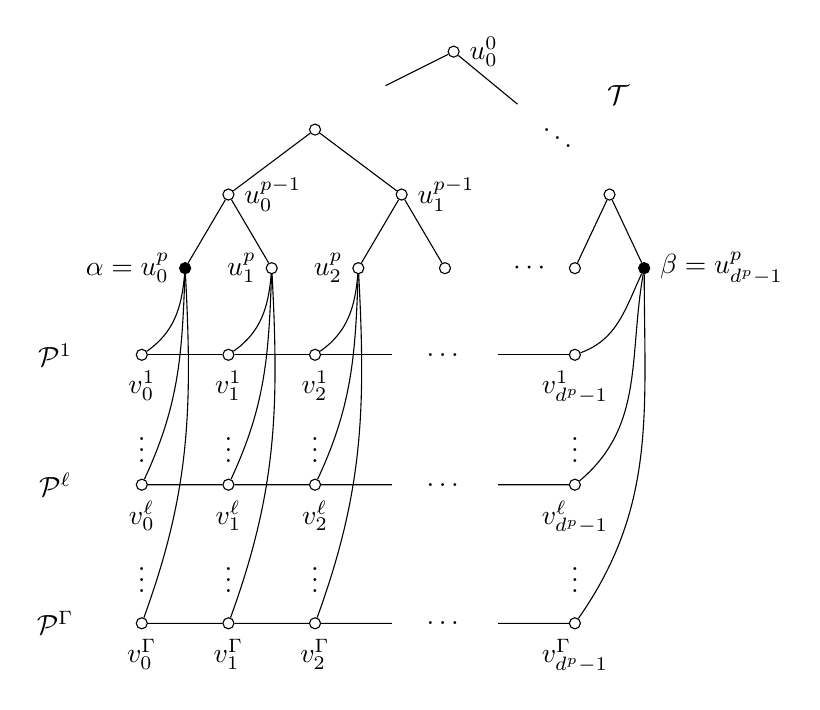
\begin{tikzpicture}[scale=1.1]
    % Define styles for different types of vertices
    \tikzset{
        vertex/.style={circle, draw, minimum size=4pt, inner sep=1pt, fill=white},
        filled/.style={circle, draw, fill=black, minimum size=4pt, inner sep=1pt},
    }
    
    
    % Draw vertices on level A with labels
    \node[] at (-1,0) {$\mathcal{P}^1$};
    \node[vertex] (a) at (0,0) [label=below:$v^1_0$] {};
    \node[vertex] (b) at (1,0) [label=below:$v^1_1$] {};
    \node[vertex] (c) at (2,0) [label=below:$v^1_2$] {};
    \node[] (ca) at (3,0) {};
    \node[] at (3.5,0) {$\dots$};
    \node[] (cb) at (4,0) {};
    \node[vertex] (d) at (5,0) [label=below:$v^1_{d^p-1}$] {};

    \node (dda) at (0,-1) {$\vdots$};
    \node (ddb) at (1,-1) {$\vdots$};
    \node (ddc) at (2,-1) {$\vdots$};
    \node (ddd) at (5,-1) {$\vdots$};
    \node (ddda) at (0,-2.5) {$\vdots$};
    \node (dddb) at (1,-2.5) {$\vdots$};
    \node (dddc) at (2,-2.5) {$\vdots$};
    \node (dddd) at (5,-2.5) {$\vdots$};
    
    % Draw vertices on level B with labels
    \node[] at (-1,-1.5) {$\mathcal{P}^\ell$};
    \node[vertex] (e) at (0,-1.5) [label=below:$v^\ell_0$] {};
    \node[vertex] (f) at (1,-1.5) [label=below:$v^\ell_1$] {};
    \node[vertex] (g) at (2,-1.5) [label=below:$v^\ell_2$] {};
    \node[] (ga) at (3,-1.5) {};
    \node[] at (3.5,-1.5) {$\dots$};
    \node[] (gb) at (4,-1.5) {};
    \node[vertex] (h) at (5,-1.5) [label=below:$v^\ell_{d^p-1}$] {};
    
    % Draw vertices on level C with labels
    \node[] at (-1,-3.1) {$\mathcal{P}^\Gamma$};
    \node[vertex] (i) at (0,-3.1) [label=below:$v^\Gamma_0$] {};
    \node[vertex] (j) at (1,-3.1) [label=below:$v^\Gamma_1$] {};
    \node[vertex] (k) at (2,-3.1) [label=below:$v^\Gamma_2$] {};
    \node[] (ka) at (3,-3.1) {};
    \node[] at (3.5,-3.1) {$\dots$};
    \node[] (kb) at (4,-3.1) {};
    \node[vertex] (l) at (5,-3.1) [label=below:$v^\Gamma_{d^p-1}$] {};
    
    % Draw tree structure vertices
    \node at (5.5,3) {$\mathcal{T}$};
    \node[vertex] (o) at (3.6,3.5) [label=right:$u_0^0$] {};
    
    \node (left) at (2.7,3.05) {};
    \node (right) at (4.45,2.8) {};
    
    \node (eleft) at (2.45,3) {$\iddots$};
    \node (eright) at (4.8,2.6) {$\ddots$};
    \node[vertex] (pq) at (2,2.6) {};
    
    \node[vertex] (p) at (1,1.85) [label=right:$u^{p-1}_0$] {};
    \node[vertex] (q) at (3,1.85) [label=right:$u^{p-1}_1$] {};
    \node[vertex] (qq) at (5.4,1.85) {};
    
    \node[filled] (s) at (0.5,1) [label=left:{$\alpha=u^p_0$}] {};
    \node[vertex] (m) at (1.5,1) [label=left:$u^p_1$] {};
    \node[vertex] (n) at (2.5,1) [label=left:$u^p_2$] {};
    \node[vertex] (nn) at (3.5,1) {};
    \node (mid) at (4.5,1) {$\cdots$};
    \node[vertex] (rl) at (5,1) {};
    \node[filled] (r) at (5.8,1) [label=right:{$\beta=u^p_{d^p-1}$}] {};
    
    % Draw path connections
    \draw (a) -- (b) -- (c) -- (ca);
    \draw (e) -- (f) -- (g) -- (ga);
    \draw (i) -- (j) -- (k) -- (ka);
    \draw (cb) -- (d);
    \draw (gb) -- (h);
    \draw (kb) -- (l);
    
    % Draw tree connections
    \draw (o) -- (left);
    \draw (o) -- (right);
    \draw (p) -- (pq);
    \draw (q) -- (pq);
    \draw (p) -- (s);
    \draw (p) -- (m);
    \draw (q) -- (n);
    \draw (q) -- (nn);
    \draw (qq) -- (r);
    \draw (qq) -- (rl);
    
    \draw (s) to [out=265, in=35] (a);
    \draw (s) to [out=268, in=65] (e);
    \draw (s) to [out=273, in=70] (i);
    \draw (m) to [out=265, in=35] (b);
    \draw (m) to [out=268, in=65] (f);
    \draw (m) to [out=273, in=70] (j);
    \draw (n) to [out=265, in=35] (c);
    \draw (n) to [out=268, in=65] (g);
    \draw (n) to [out=273, in=70] (k);
    \draw (r) to [out=245, in=20] (d);
    \draw (r) to [out=260, in=40] (h);
    \draw (r) to [out=270, in=55] (l);
\end{tikzpicture}
    \caption{An example of $\GGdp$ with $d=2$.}
    \label{fig:GGdp}
\end{figure}

We restate the simulation lemma of \citet{das2011distributed}, which connects the computation of Boolean function in the traditional communication complexity model to the computation of Boolean function in the distributed model in graph $\GGdp$ with input vertices $\alpha$ and $\beta$.


% \yanyu{maybe the lemma before the simulation lemma is also needed. (will add later if it's needed)}
\begin{lemma}[Simulation lemma \cite{das2011distributed}]
\label{thm:simulation}
For any $\Gamma$, $d$, $p$, $B$, $\epsilon\geq 0$, and function $f:\bin^b \times \bin^b \to \bin$, if there is an $\epsilon$-error randomized distributed algorithm that computes $f(x,y)$ faster than $\frac{d^p-1}{2}$ rounds on $\GGdp$ with $x$ given to vertex $\alpha$ and $y$ given to vertex $\beta$, i.e.,
$
R_\epsilon^{\GGdp}(f) < \frac{d^p-1}{2},
$
then there is an $\epsilon$-error randomized algorithm in the communication complexity model that computes $f$ using at most $2dpB R_\epsilon^{\GGdp}(f)$ bits of communication.
In other words,
$
R_\epsilon^{cc-pub}(f)\leq 2dpB R_\epsilon^{\GGdp}(f).
$
% \yijun{When I first read the theorem I found it very confusing. I think an important point that is missing is that you need to say how the input to the function $f$ is stored in the network.}
\end{lemma}
%\yijun{rounds in distributes setting, bits in communication complexity}

% The simulation lemma was proved by carefully analyzing the states of the distributed (sub)-network over rounds, and showing that only $O(dp)$ messages are needed for Alice and Bob to simulate one round of the execution of any distributed algorithm on $\GGdp$. Hence, Alice and Bob can perform the above simulation and run any distributed algorithm for computing functions on $\alpha$ and $\beta$ on $\GGdp$ in the communication complexity model with only $O(dp)$-factor overhead.

% \yijun{Some suggestions: 
% (1) Include a very brief proof idea for the simulation lemma. 
% (2) Include a very brief proof sketch (no theorems, just a paragraph) for how the simulation lemma is used to give $\Omega(\sqrt{n})$ for one problem. Otherwise, the reader might be very lost.
% }
% \yanyu{(1) above (2) below}
The simulation lemma was proved by analyzing the states of the distributed (sub)-network over rounds. In $\GGdp$, Alice and Bob have two ways to communicate $b$ bits: either through paths of length $d^p-1$ between them, or through the tree structure. When an algorithm's runtime is less than $(d^p-1)/2$, messages cannot traverse the full path between Alice and Bob, forcing communication through the tree structure. This creates a congestion bottleneck which is manifested by their analysis that only $O(dp)$ messages are needed to simulate all messages sent in each round of the distributed algorithm on $\GGdp$. This allows Alice and Bob to simulate any distributed algorithm for computing functions $f$ on $\alpha$ and $\beta$ on $\GGdp$ in the communication complexity model with an $O(dp)$-factor overhead.
%\yanyu{edited}
%\yijun{the paragraph above essentially conveys zero information... I would at least explain why the threshold $(d^p-1)/2$ makes sense: Essentially there are two ways for Alice and Bob to communicate $\Theta(d^p)$ bits of information to each other: via paths or via trees, the first suffers from a dilation of $\Theta(d^p)$, the second suffers from a congestion of $\Theta(d^p)$}

The main way the above simulation lemma is used is via the following lemma which applies the simulation lemma specifically for the $\disj$ function. It translates the lower bound for $\disj$ in the communication model to a lower bound for computing $\disj$ in $\GGdp$ on $\alpha$ and $\beta$. 

\begin{lemma}[Set disjointness lower bound for $\GGdp$~\cite{das2011distributed}]\label{lem:disj}
For any $\Gamma, d, p$, there exists a constant $\epsilon>0$ such that
$$R_\epsilon^{\GGdp}\left(\disj_b;B\right)=\Omega\left(\min\left(d^p, \frac{b}{dpB}\right)\right).$$
\end{lemma}






\subsection{Modification to \GGdptitle{}}
\label{subsec:modification}

In this section, we present our graph construction $\Gkdpp$ builds upon $\GGdp$ to allow us to perform a reduction from distributed set disjointness to the \secsisp{} and \rpath{} problems. Compared with the $\widetilde{\Omega}(\sqrt{n})$ lower bounds obtained via existing constructions~\cite{das2011distributed,manoharan2024computing}, our graph construction $\Gkdpp$ allows us to obtain a higher $\widetilde{\Omega}(n^{2/3})$ lower bound. 
%\yijun{the first sentence is a bit awkward}
We show how to simulate any distributed disjointness algorithm for $\Gkdpp$ on $\GGdp$ with $O(1)$-factor overhead. Connecting these two results, we obtain a lower bound for computing disjointness on $\Gkdpp$ with inputs given to $\alpha$ and $\beta$.

\paragraph{Intuition.} Our lower bound construction is built around a bipartite graph positioned at the far end of the structure, which controls the replacement path distances for each edge along the given $s$-$t$ path. We aim to establish a correspondence between the edge orientations in the bipartite graph and the replacement path distances for the edges in the given $s$-$t$ path. Moreover, we require that reversing the orientation of the edges in the bipartite graph result in longer replacement paths. To solve the replacement path problem, Alice must learn the orientation of every edge in the bipartite graph, requiring substantial information to be transmitted from one end to the other.
%\yanyu{edited}
% so that the length of the second simple shortest path, i.e. the minimum replacement path across all edges in the given $s$-$t$ path, can be used to indicate the disjointness between two parties. 
% \yanyu{is this confusing out of context?}
% \yijun{This is confusing because You only discuss $M$ and omit $x$ entirely. There are two ways to improve the writing: One is that here you just say that to solve replacement paths we need to learn all the edge orientations in the bipartite graphs (without mentioning \secsisp{} and set disjointness), requiring transmitting a lot of information from one end to the other end. Second is to include more detail of not only $M$ but also $x$ and say that they correspond to the set disjointness input and how they affect replacement path length (you can also choose to do this later in the place where you introduce them).}

The construction proceeds by first establishing a mapping between each edge on the $s$-$t$ path and its corresponding edge in the bipartite graph. 
For each edge in the $s$-$t$ path, we connect a long path to its mapped edge in the bipartite graph.
% to increase the distance between the given $s$-$t$ path and the bipartite graph where the direction information is stored. 
The long distance between the output vertices (vertices in the given $s$-$t$ path) and the location of critical information (edge orientations in the bipartite graph) forces the algorithm to spend more rounds propagating information to their required destinations. 
The orientation of the edges in the bipartite graph determines the length of the replacement path for their corresponding edges. %This correspondence is critical for computing disjointness. 
With $n^{1/3}$ paths of length approximately $n^{2/3}$, the algorithm requires at least $n^{2/3}$ rounds to propagate this critical information. 
Next, to reduce the graph's diameter without creating additional replacement paths, we incorporate a tree-like structure with downward edge orientations along the path. As demonstrated in the simulation lemma of \citet{das2011distributed} and our new simulation in \Cref{lem:disj G(kdpp)}, this structure does not substantially improve the propagation of critical information.
Finally, to optimize the total number of vertices, we carefully merge paths that lead to the same vertex in the bipartite graph while ensuring that the correspondence between edge orientations in the bipartite graph and replacement path lengths remains intact.
%\yanyu{edited}
% \yijun{I did not see the main idea being explicitly mentioned: the orientation of each edge in the bipartite graph controls the replacement path length for the corresponding edge (for one direction, you can use that in the replacement path, for the other direction, you need to take a longer detour), so the replacement path distance can be used to determine the direction of the corresponding edge in the bipartite graph. Therefore, solving the replacement path problem requires communicating $\Omega(n^{2/3})$ bits of information from one side of the graph to the other side of the graph.}


\paragraph{Construction of \Gkdpptitle.}
Our modified graph is called $\Gkdpp$ where $\phi: [k^2] \to [k]\times[k]$ is a bijection used to map any edge $\left(s_{i-1}, s_i\right)$ on the given $s$-$t$ path to an edge on the bipartite graph. Refer to \Cref{fig:Gkdpp} for an illustration. We present the construction of $\Gkdpp$ with some default edge orientation. %If the problem in consideration only concerns undirected graph, then ignore the default direction provided. [Yi-Jun: I commented out the above sentence as it seems irrelevant to us]
The graph $\Gkdpp$ is constructed via the following steps:
% \yijun{
% This is a complicated construction. Need to give intuition. Also, 
% try to give a proof sketch/idea before presenting the formal proofs in the next sub-section.}
\begin{enumerate}
    \item Construct $\GGdp$ with $\Gamma = 2k$. We relabel the vertices of the last $k$ paths by $w^\ell_i$, where $1\leq\ell\leq k$ and $0\leq i\leq d^p-1$. For $1\leq\ell\leq k$, we use the shorthand $v^\ell$ and $w^\ell$ to denote the \emph{last} vertex of path $\Pc^\ell$ and $\Pc^{\ell+k}$, respectively. 
    \item For $1\leq i,j \leq k$, add edges $\{v^i, w^j\}$.
    \item Add a directed path $\mathcal{P^*}$ with $k^2$ edges from $s$ to $t$.\\ We label the vertices on the path by $s=s_0, s_1, \dots, s_{k^2}=t$. 
    \item Add $k$ paths $\Qc^1, \dots, \Qc^k$ each of length $2k^2$, where $\Qc^\ell$ consists of vertices $q^\ell_0, \dots, q^\ell_{2k^2}$. \\For each $1\leq\ell\leq k$, add edge $\left(q^{\ell}_{2k^2}, v^{\ell}_0\right)$.
    \item Add $k$ paths $\Rc^1, \dots, \Rc^k$ each of length $2k^2$, where $\Rc^\ell$ consists of vertices $r^\ell_0, \dots, r^\ell_{2k^2}$. \\For each $1\leq\ell\leq k$, add edge $\left(w^{\ell}_0, r^{\ell}_{0}\right)$.
    \item For $i\in [k^2]$, suppose $\phi(i)=\left(\phi_1(i),\phi_2(i)\right)$, add $\left\{s_{i-1}, q^{\phi_1(i)}_{2(i-1)}\right\}$ and $\left(r^{\phi_2(i)}_{2i}, s_i\right)$.
    \item Add edges from $\alpha$ to all vertices in $\Pstar, \Qc^i, \Rc^i$, for each $1\leq i \leq k$.
\end{enumerate}

\paragraph{Direction of edges.}
To facilitate our reduction from set disjointness to \secsisp{}, we assigned default orientations for all edges in $\Gkdpp$ except for those in the right bipartite graph and edges of the form $\left\{s_{i-1}, q^{\phi_1(i)}_{2(i-1)}\right\}$. The direction of the edges on the bipartite graph is determined by a matrix $M\in \bin^{k\times k}$ and the direction of the edges $\left\{s_{i-1}, q^{\phi_1(i)}_{2(i-1)}\right\}$ are determined by a vector $x\in \bin^{k^2}$. The directed version of the graph $\GkdppMx$ is constructed as follows.

\begin{enumerate}
    \item Orient the edges in paths $\Pstar, \Pc^\ell, \Qc^\ell, \Rc^\ell$ pointing to larger index for $1\leq \ell \leq k$ and orient the edges in paths $\Pc^\ell$ pointing to smaller index for $k+1\leq \ell \leq 2k$.
    \item Orient the edges in the tree $\Tc$ from parents to children. Orient the edges between the leaves and the paths pointing away from the leaves.  
    \item For $1\leq i,j \leq k$, add edge $(v^i, w^j)$ if $M_{ij}=1$. Otherwise, add edge $(w^j, v^i)$.
    \item For $i\in [k^2]$, set direction as $\left(s_{i-1}, q^{\phi_1(i)}_{2(i-1)}\right)$ if $x_i = 1$. Otherwise, set direction as $\left(q^{\phi_1(i)}_{2(i-1)}, s_{i-1}\right)$.
\end{enumerate}

When $x_i = 1$, alternative paths avoiding $\left(s_{i-1}, s_i\right)$ can use the edge $\left(s_{i-1}, q^{\phi_1(i)}_{2(i-1)}\right)$ to make a detour. Conversely, when $x_i = 0$, any alternative paths avoiding $(s_{i-1}, s_i)$ must leave $\Pstar$ before $s_{i-1}$. Since the paths $\Qc^\ell$ have double the length, alternative paths exiting earlier will have longer lengths. If the corresponding edge in the bipartite graph is oriented as $\left(v^{\phi_1(i)}, w^{\phi_2(i)}\right)$ (i.e. when $M_{\phi_1(i), \phi_2(i)}=1$), the returning detour using the edge $\left(r^{\phi_2(i)}_{2i}, s_i\right)$ can be taken. For the same reason, detours returning earlier will have shorter lengths. Hence, the shortest detour is possible if and only if both $x_i = 1$ and $M_{\phi_1(i), \phi_2(i)}=1$, allowing us to reduce set disjointness to \secsisp{}.

%\yanyu{added motivation behind $M$ and $x$}
% \yijun{Now is the right place to explain the motivation behind $M$ and $x$: Say that they correspond to the set disjointness input, and intuitively how their values affect replacement path length.}
% Firstly, we consider $\Gamma = 2k$ and we relabel the vertices of the last $k$ path as $w^\ell_i$. Now, we add a directed path $\mathcal{P^*}$ with $k^2$ edges from $s$ to $t$. We label the vertices on the path by $s=s_0, s_1, \dots, t=s_{k^2}$. 
% Then consider a bijection $\phi: [k^2] \to [k]\times[k]$. Suppose $\phi(i) = (\phi(i)_1, \phi(i)_2)$, this bijection is used to map any edge $\left(s_{i-1}, s_i\right)$ on $\Pstar$ to a vertex pair $\left(v^{\phi(i)_1}, w^{\phi(i)_2}\right)$. 
% Then we further add $2k$ number of paths $\Qc^1, \dots, \Qc^k$ and $\Rc^1, \dots, \Rc^k$, each having $2k^2$ edges, with vertices indexed from $0$ to $2k^2$. For each $1\leq\ell\leq k$, add edges $\left(q^{\ell}_{2k^2}, v^{\ell}_0\right)$ and $\left(w^{\ell}_0, r^{\ell}_{0}\right)$
% For each edge $(s_{i-1}, s_i)$, add $\left(s_{i-1}, q^{\phi(i)_1}_{2(i-1)}\right)$ and $\left(r^{\phi(i)_2}_{2i}, s_i\right)$. Lastly, we add edges from $\alpha$ to all vertices on $\Pstar, \Qc^i, \Rc^i$.


\begin{figure}[ht!]
    \centering
    \begin{tikzpicture}[scale=1.1]
\scriptsize
    % Define styles for different types of vertices
    \tikzset{
        vertex/.style={circle, draw, minimum size=4pt, inner sep=1pt, fill=white},
        filled/.style={circle, draw, fill=black, minimum size=4pt, inner sep=1pt},
        symbol/.style={inner sep=0pt, font=\small, text height=12pt},
        small/.style={font=\small},
        mapping/.style={teal!60!blue, thick},
        dir/.style={arrows = {-Stealth[inset=0.7pt, length=5pt, angle'=25]}},
        widedir/.style={arrows = {-Stealth[inset=0.7pt, length=5pt, angle'=35]}},
        highlight/.style={teal!70!green, thick},
        hlar/.style={highlight, dir},
        line/.style={gray, very thin, dir},
    }
    
    % Draw vertices on level A with labels
    \node[] at (-0.4,0) {$\mathcal{P}^1$};
    \node[vertex] (a) at (0,0) [label=below:$v^1_0$] {};
    \node[vertex] (b) at (1,0) [label=below:$v^1_1$] {};
    \node[vertex] (c) at (2,0) [label=below:$v^1_2$] {};
    \node[] (ca) at (3.5,0) {};
    % \node[] (ca2) at (3.5,0) {};
    \node[small] at (4,0) {$\cdots$};
    \node[] (cb) at (4.5,0) {};
    \node[vertex] (d) at (7.5,0) [label=right:{$v^1=v^1_{d^p-1}$}] {};

    \node[symbol] (dda) at (0,-0.7) {$\vdots$};
    \node[symbol] (ddb) at (1,-0.7) {$\vdots$};
    \node[symbol] (ddc) at (2,-0.7) {$\vdots$};
    \node[symbol] (ddd) at (6.6,-0.6) {$\iddots$};
    
    \node[symbol] (ddda) at (0,-3.8) {$\vdots$};
    \node[symbol] (dddb) at (1,-3.8) {$\vdots$};
    \node[symbol] (dddc) at (2,-3.8) {$\vdots$};
    \node[symbol] (dddd) at (6.6,-3.4) {$\ddots$};
    
    % Draw vertices on level B with labels
    \node[] at (-0.4,-1.2) {$\mathcal{P}^k$};
    \node[vertex] (e) at (0,-1.2) [label=below:$v^k_0$] {};
    \node[vertex] (f) at (1,-1.2) [label=below:$v^k_1$] {};
    \node[vertex] (g) at (2,-1.2) [label=below:$v^k_2$] {};
    \node[] (ga) at (3.5,-1.2) {};
    \node[small] at (4,-1.2) {$\cdots$};
    \node[] (gb) at (4.5,-1.2) {};
    \node[vertex] (h) at (6,-1.2) [label=below left:{$v^k$}] {};

    % Draw vertices on level C with labels
    \node[] at (-0.5,-2.8) {$\mathcal{P}^{k+1}$};
    \node[vertex] (e2) at (0,-3) [label=below:$w^1_0$] {};
    \node[vertex] (f2) at (1,-3) [label=below:$w^1_1$] {};
    \node[vertex] (g2) at (2,-3) [label=below:$w^1_2$] {};
    \node[] (ga2) at (3.5,-3) {};
    \node[small] at (4,-3) {$\cdots$};
    \node[] (gb2) at (4.5,-3) {};
    \node[vertex] (h2) at (6,-3) [label=below:{$w^1$}] {};
    
    
    % Draw vertices on level D with labels
    \node[] at (-0.5,-4) {$\mathcal{P}^{2k}$};
    \node[vertex] (i) at (0,-4.2) [label=below:$w^k_0$] {};
    \node[vertex] (j) at (1,-4.2) [label=below:$w^k_1$] {};
    \node[vertex] (k) at (2,-4.2) [label=below:$w^k_2$] {};
    \node[] (ka) at (3.5,-4.2) {};
    \node[small] at (4, -4.2) {$\cdots$};
    \node[] (kb) at (4.5,-4.2) {};
    \node[vertex] (l) at (7.5,-4.2) [label=below:{$w^k=w^k_{d^p-1}$}] {};
    
    % Draw tree structure vertices
    \begin{scope}[xshift=1.5mm, yshift=0mm]
        \node at (5,3) {$\mathcal{T}$};
        \node[vertex] (o) at (3.3,3.6) [label=right:$u_0^0$] {};
        
        \node (left) at (2.7,3.2) {};
        \node (right) at (4.1,3.0) {};
        
        \node[symbol] (eleft) at (2.4,3.1) {$\iddots$};
        \node[symbol] (eright) at (4.5,2.7) {$\ddots$};
        \node[small] (mid) at (4,1) {$\cdots$};
        \node[vertex] (pq) at (2,2.8) {};
        
        \node[vertex] (p) at (1,2) [label=right:$u^{p-1}_0$] {};
        \node[vertex] (q) at (2.9,2) [label=right:$u^{p-1}_1$] {};
        \node[vertex] (qq) at (5.1,2) {};
        
        \node[filled] (s) at (0.5,) [label=above left:{$\alpha=u^p_0$}] {};
        \node[vertex] (m) at (1.5,1) [label=left:$u^p_1$] {};
        \node[vertex] (n) at (2.5,1) [label=left:$u^p_2$] {};
        \node[vertex] (nn) at (3.3,1) {};
        \node[vertex] (rl) at (4.7,1) {};
        \node[filled] (r) at (5.5,1) [label=above right:{$\beta=u^p_{d^p-1}$}] {};
    \end{scope}
    % Draw path connections
    \draw[dir, highlight] (a) -- (b) -- (c) -- (ca);
    \draw[dir] (e) -- (f) -- (g) -- (ga);
    \draw[dir] (ga2) -- (g2) -- (f2) -- (e2);
    \draw[dir, highlight] (ka) -- (k) -- (j) -- (i);
    \draw[dir, highlight] (cb) -- (d);
    \draw[dir] (gb) -- (h);
    \draw[dir] (h2) -- (gb2);
    \draw[dir, highlight] (l) -- (kb);
    
    % Draw tree connections
    \draw[line] (o) -- (left);
    \draw[line] (o) -- (right);
    \draw[line] (pq) -- (p);
    \draw[line] (pq) -- (q);
    \draw[line] (p) -- (s);
    \draw[line] (p) -- (m);
    \draw[line] (q) -- (n);
    \draw[line] (q) -- (nn);
    \draw[line] (qq) -- (r);
    \draw[line] (qq) -- (rl);
    
    \draw[line] (s) to [out=269,in=35] (a);
    \draw[line] (s) to [out=269,in=50] (e);
    \draw[line] (s) to [out=272,in=60] (e2);
    \draw[line] (s) to [out=275,in=60] (i);
    
    \draw[line] (m) to [out=269,in=35] (b);
    \draw[line] (m) to [out=269,in=50] (f);
    \draw[line] (m) to [out=272,in=60] (f2);
    \draw[line] (m) to [out=275,in=60] (j);
    
    \draw[line] (n) to [out=268,in=35] (c);
    \draw[line] (n) to [out=269,in=50] (g);
    \draw[line] (n) to [out=272,in=60] (g2);
    \draw[line] (n) to [out=275,in=60] (k);
    
    \draw[line] (r) to [out=355,in=115] (d);
    \draw[line] (r) to [out=300,in=85] (h);
    \draw[line] (r) to [out=260,in=120, looseness=1] (h2);
    \draw[line] (r) to [out=258,in=175, looseness=1.2] (l);

    % Bipartite graph mapped from the string y
    \node (vl) at (6.95,-0.25) {};
    \node (wl) at (6.95,-3.85) {};
    \draw[dir, mapping] (d) -- (h2);
    \draw[dir, mapping] (d) -- (wl);
    \draw[dir, mapping] (vl) -- (l);
    \draw[dir, mapping] (wl) -- (vl);
    \draw[dir, mapping] (vl) -- (h2);
    \draw[dir, mapping] (h) -- (l);
    \draw[dir, mapping] (h2) -- (h);
    \draw[dir, mapping] (wl) -- (h);
    \draw[widedir, highlight, very thick] (d) -- (l);

    \begin{scope}[xshift=-35mm, yshift=-1mm]
        \node[vertex] (s0) at (0,-4) [label=left:{$s=s_0$}] {};
        \node[vertex] (s1) at (0,-3) [label=left:$s_1$] {};
        \node[symbol] (s2) at (0,-2) {$\vdots$};
        \node[vertex] (sj) at (0,-1) [label=below left:$s_{i-1}$] {};
        \node[vertex] (si) at (0,0) [label=below left:$s_i$] {};
        \node[symbol] (s5) at (0,1) {$\vdots$};
        \node[vertex] (st) at (0,2) [label=below left:{$t=s_{k^2}$}] {};
        \node[symbol] (Pstar) at (-0.1,2.52)  {$\mathcal{P}^*$};

        \draw[dir, highlight] (s0) -- (s1);
        \draw[dir, highlight] (s1) -- (s2);
        \draw[dir, highlight] (s2) -- (sj);
        \draw[dir, red, thick] (sj) -- (si);
        \draw[dir, highlight] (si) -- (s5);
        \draw[dir, highlight] (s5) -- (st);

        \node[symbol] (Q)  at (1.2,2.5)    {$\mathcal{Q}^1$};
        \node[vertex] (q0)  at (1.3,-4)     [label=right:{$q^1_0$}] {};
        \node[vertex] (q05) at (1.3,-3.5) [label=right:{$q^1_1$}] {};
        \node[vertex] (q1)  at (1.3,-3)    [label=right:{$q^1_2$}] {};
        \node[symbol] (q2)  at (1.3,-2) {$\vdots$};
        \node[vertex] (qj)  at (1.3,-1)    [label=below right:$q^1_{2i-2}$]{};
        \node[vertex] (qji) at (1.3,-0.5) [label=right:$q^1_{2i-1}$]{};
        \node[vertex] (qi)  at (1.3,0)     [label=right:$q^1_{2i}$] {};
        \node[symbol] (q5)  at (1.3,1) {$\vdots$};
        \node[vertex] (qt)  at (1.3,2)     [label=below right:{$q^1_{2k^2}$}] {};

        \draw[dir] (q0)  -- (q05);
        \draw[dir] (q05) -- (q1);
        \draw[dir] (q1)  -- (q2);
        \draw[dir] (q2)  -- (qj);
        \draw[dir, highlight] (qj)  -- (qji);
        \draw[dir, highlight] (qji) -- (qi);
        \draw[dir, highlight] (qi)  -- (q5);
        \draw[dir, highlight] (q5)  -- (qt);

        \node[symbol] (r)  at (-1.5,2.55)    {$\mathcal{R}^k$};
        \node[vertex] (r0)  at (-1.5,-4)    [label=left:{$r^k_0$}] {};
        \node[vertex] (r05) at (-1.5,-3.5)  [label=left:{$r^k_1$}] {};
        \node[vertex] (r1)  at (-1.5,-3)    [label=left:{$r^k_2$}] {};
        \node[symbol] (r2)  at (-1.5,-2) {$\vdots$};
        \node[vertex] (rj)  at (-1.5,-1)    [label=left:$r^k_{2i-2}$]{};
        \node[vertex] (rji) at (-1.5,-0.5)  [label=left:$r^k_{2i-1}$]{};
        \node[vertex] (ri)  at (-1.5,0)     [label=above left:$r^k_{2i}$] {};
        \node[symbol] (r5)  at (-1.5,1) {$\vdots$};
        \node[vertex] (rt)  at (-1.5,2)     [label=below left:{$r^k_{2k^2}$}] {};

        \draw[dir, highlight] (r0)  -- (r05);
        \draw[dir, highlight] (r05) -- (r1);
        \draw[dir, highlight] (r1)  -- (r2);
        \draw[dir, highlight] (r2)  -- (rj);
        \draw[dir, highlight] (rj)  -- (rji);
        \draw[dir, highlight] (rji) -- (ri);
        \draw[dir] (ri)  -- (r5);
        \draw[dir] (r5)  -- (rt);
        
        \draw[hlar] (ri)  to [out=20,in=165] (si);
        \draw[hlar] (sj)  to [out=345,in=200] (qj);
    \end{scope}

    \draw[dir, highlight] (qt)  to [out=30,in=120] (a);
    \draw[dir, highlight] (i)  to [out=200,in=320] (r0);
    \node[symbol] (PPP)  at (-1.5,-5) {{\color{teal!70!green}$P$}};
\end{tikzpicture}
    \caption{Illustration of $\Gkdpp$, assuming $\phi(i)=(1,k)$ and $M_{1,k} = 1$. Paths $\Qc^2,\dots,\Qc^k$ and $\Rc^1,\dots,\Rc^{k-1}$ are omitted. Other edges from $\Pstar$ to $\Qc^1$, and from $\Rc^k$ to $\Pstar$ are omitted. Edges from $\alpha$ to $\Pstar, \Qc^i$ and $\Rc^i$ are omitted. Reversed directional edges in the bipartite graph are omitted. When $(v^1, w^k)$ is oriented correctly, the green highlighted path $P$ is a replacement path from $s$ to $t$ for the deleted edge $(s_{i-1}, s_i)$.}
    \label{fig:Gkdpp}
\end{figure}

\begin{observation}[Basic properties of $\Gkdpp$]\label{obs:Gkdpp}
    There are $\Theta(k^3 + k d^p)$ vertices in $\Gkdpp$, and the diameter of $\Gkdpp$ is at most $2p+2$.
\end{observation}
    % \yijun{add a very short proof: especially the diameter part.}

\begin{proof}
    The number of vertices for the respective parts are: $2k d^p$ vertices for $\Pc^\ell$, $2k \times (2k^2+1)$ for $\Rc^\ell$ and $\Qc^\ell$, $k^2+1$ vertices for $\Pstar$ and $\frac{d^{p+1}-1}{d-1}$ vertices for $\Tc$. Hence the total number of vertices is $2k d^p +4k^3 + 2k + k^2 + 1 + \frac{d^{p+1}-1}{d-1} = \Theta(k^3+kd^p)$. Every vertex not on the tree $\Tc$ is connected to some leaf in $\Tc$. Since $\Tc$ has depth $p$, the diameter of $\Gkdpp$ is at most $2p+2$.
\end{proof}
    
Now we show a lemma for a lower bound of distributed algorithms for set disjointness on $\Gkdpp$. This is analogous to \Cref{lem:disj}. We achieve this by applying \Cref{thm:simulation} and \Cref{lem:disj} in a black-box manner, and showing how distributed algorithms for set disjointness on $\Gkdpp$ can be simulated on $\GGdp$ with $O(1)$-factor overhead. The intuition for the simulation is that $\alpha$ will simulate the vertices in $\Pstar, \Qc^\ell$ and $\Rc^\ell$ and $\beta$ will simulate the vertices in the bipartite graph. 


% \begin{theorem}[simulation lemma II]
% \label{thm:simulation G(kdpp)}
% For any $k$, $d$, $p$, $B$, bijection $\phi: [k^2]\to [k]\times [k]$ and matrix $M \in \bin^{k\times k}$,
% any $T$-round distributed algorithm $\Ac$ on $\Gkdpp$ can be simulated in $\GGdp$, with $\Gamma=2k$ in $3T$ rounds.
% \end{theorem}
% \yanyu{do we need to say what do we mean by ``simulate'' or is it clear in this context?}
% \yijun{I think you can avoid this issue by removing this theorem and incorporating the proof into the lemma below.}


% \begin{proof}
    
% \end{proof}


\begin{lemma}[Set disjointness lower bound for $\Gkdpp$]
\label{lem:disj G(kdpp)}
    For any $k, d, p$ and bijection $\phi: [k^2]\to [k]\times [k]$ there exists a constant $\epsilon>0$ such that
    $$R_\epsilon^{\Gkdpp}\left(\disj_b;B\right)=\Omega\left(\min\left(d^p, \frac{b}{dpB}\right)\right).$$
\end{lemma}

\begin{proof}
    First, we show that if there is a $T$-round distributed algorithm for set disjointness $\Ac$ on $\Gkdpp$, then there is a $3T$-round distributed algorithm for set disjointness on $\GGdp$. We achieve this via simulating $\Ac$ on $\GGdp$.

    Suppose we have an algorithm $\Ac$ on graph $\GkdppMx$, we will denote a message sent in the $i$th round of $\Ac$ from vertex $u$ to vertex $v$ as $\Mc_i(u\to v)$. 
    Now $\alpha$ in $\GGdp$ can simulate all the vertices in $\Rc^\ell, \Qc^\ell$ and $\Pstar$ in the following way. 
    vertex $\alpha$ will run $2k+2$ processes and run $\Ac$ for $\alpha, \Rc^\ell, \Qc^\ell$ and $\Pstar$ for $1\leq \ell \leq k$ on these processes. 
    Any messages among the vertices in $\alpha, \Rc^\ell, \Qc^\ell$ and $\Pstar$ can be handled locally between the processes.
    The only messages left are between $v^\ell_0$ and $q^\ell_{2k^2}$ and between $w^\ell_0$ and $r^\ell_0$, where $1\leq \ell\leq k$. For each $1\leq \ell\leq k$, $\Mc_i(q^\ell_{2k^2}\to v^\ell_0)$ and $\Mc_i(v^\ell_0 \to q^\ell_{2k^2})$ are delivered along the edge $\{q^\ell_{2k^2}, v^\ell_0\}$. Similarly, $\Mc_i(r^\ell_{0}\to w^\ell_0)$ and $\Mc_i(w^\ell_0 \to r^\ell_{0})$ are delivered along the edge $\{r^\ell_{0}, w^\ell_0\}$.  
    Since there are at most twice the number of messages along the edges of $\alpha$, we can simulate $\Ac$ on $\GGdp$ in $3T$ rounds.

    Now we describe how to handle the bipartite graph in $\GkdppMx$ in vertex $\beta$ on $\GGdp$. vertex $\beta$ will create $2k+1$ processes that run $\Ac$ acting as $\beta, v^\ell$ and $w^\ell$ locally, where $1\leq \ell\leq k$. Any messages among these vertices are handled locally on $\beta$. The only messages left are between $v^\ell_{d^p-2}$ and $v^\ell$ and between $w^\ell_{d^p-2}$ and $w^\ell$. We will focus on $v^\ell$ now since the behaviors on $w^\ell$ are similar. In the $(3i-2)$th round, vertex $v^\ell_{d^p-2}$ and $v^\ell$ exchange $\Mc_i(v^\ell_{d^p-2}\to v^\ell)$ and $\Mc_i(v^\ell\to v^\ell_{d^p-2})$. In the $(3i-1)$th round, $v^\ell$ relay $\Mc_i(v^\ell_{d^p-2}\to v^\ell)$ to $\beta$. $\beta$ now has all the information needed to compute $\Mc_{i+1}(v^\ell \to v^\ell_{d^p-2})$ locally. $\beta$ computes $\Mc_{i+1}(v^\ell \to v^\ell_{d^p-2})$ and send it to $v^\ell$ in the $3i$th round. Now $v^\ell$ has $\Mc_{i+1}(v^\ell \to v^\ell_{d^p-2})$ to send to $v^\ell_{d^p-2}$ in the $(3(i+1)-2)$th round and the process repeats.

    All other vertices in $\GGdp$ will execute their part of $\Ac$ with $2$ empty rounds between any two rounds in $\Ac$ to align their pace with that of vertices $\alpha$ and $\beta$.
    In this way, we can simulate any $T$-round algorithm on $\GkdppMx$ with $3T$ rounds on $\GGdp$.
    
    After applying \Cref{lem:disj}, we have the desired lower bound.
\end{proof}


\subsection{Lower Bound for the \secsisp{} Problem}
\label{subsec:lower bound reduction}
%\yijun{Shorten title name}
Now we are ready to show our main results: lower bounds for the \secsisp{} problem and the \rpath{} problem. We will show \Cref{thm:2sisp lower} by a reduction from the disjointness problem on $\Gkdpp$.
Before we show a reduction from disjointness to \secsisp{}, we show a correspondence between the replacement path lengths and the edge orientations in the bipartite graph.

\begin{lemma}[Replacement path lengths]
\label{lem:GkdppMx Rpath-dir correspondence}
    Consider the graph $\GkdppMx$. For any edge $(s_{i-1},s_i)$ in the path $\Pstar$, if $M_{\phi_1(i), \phi_2(i)}=1$ and $x_i=1$, the length of the replacement path is $3k^2 + 2 d^p + 6$. Otherwise, the length is strictly greater.
\end{lemma}

\begin{proof}
    Suppose $M_{\phi_1(i), \phi_2(i)}=1$ and $x_i = 1$, then the highlighted path $P$ as shown in \Cref{fig:Gkdpp} is an alternative path. It can be easily checked that it has length $3k^2 + 2 d^p + 6$. Now we show that it is the shortest among all alternative $s$-$t$ path. Observe that all alternative $s$-$t$ path must be of the form 
    $$s, \dots, s_{j-1}, q^{\phi_1(j)}_{2j-2}, \dots, q^{\phi_1(j)}_{2k^2}, \;\Pc^{\phi_1(j)},\; \Pc^{\phi_2(l)+k}, \;r^{\phi_2(l)}_0, \dots, r^{\phi_2(l)}_{2l}, s_l,\dots, t$$ where $j\leq i$ and $l\geq i$. 
    Notice that the length of the above path is $3k^2 + 2d^p + 4 + 2(l-j+1)$. This length is minimized when $l=j=i$ and we have our highlight path $P$ with length $3k^2 + 2 d^p + 6$.

    Conversely, suppose $M_{\phi_1(i), \phi_2(i)}=0$ or $x_i=0$. If $M_{\phi_1(i), \phi_2(i)}=0$, the shortest alternative path is has length greater than $3k^2 + 2 d^p + 6$. This is because, the choice of $j=l=i$ does not constitute a directed path anymore as the bipartite edge is oriented from $w^{\phi_2(i)}$ to $v^{\phi_1(i)}$. If $x_i=0$, then the alternate $s$-$t$ path must exit $\Pstar$ before $s_{i-1}$ and therefore has length greater than $3k^2 + 2 d^p + 6$.
\end{proof}

% \yijun{I think the proof of the lemma below is ok now (up to some minor typos).}
\begin{lemma}[Reducing set disjointness to \secsisp{}]\label{lem:Disj to 2sisp}
    For any $k$, $d\geq 2$, $p$, bijection $\phi: [k^2]\to [k]\times [k]$ and $\epsilon\geq 0$, if there exists an $\epsilon$-error randomized distributed algorithm for the \secsisp{} problem on graph $\GkdppMx$ for any $M\in \bin^{k\times k}$ and any $x\in \bin^{k^2}$ then there exists an $\epsilon$-error randomized algorithm for computing $\disj_{k^2}(x,y)$ (on $k^2$-bit inputs) on $\Gkdpp$ that uses the same round complexity with additional $O(\frac{k}{B})$ rounds.
\end{lemma}

\begin{proof}
    Suppose $\Ac$ is an $\epsilon$-error randomized distributed algorithm for the \secsisp{} problem and suppose we are given a set disjointness instance with $k^2$-bit strings on $\Gkdpp$. We aim to use $\Ac$ to solve the set disjointness problem $\disj_{k^2}(x,y)$.

    Suppose Alice received $x\in \bin^{k^2}$ on vertex $\alpha$ and Bob received $y\in \bin^{k^2}$ on vertex $\beta$. By viewing $y$ as a matrix $M$ (using the lexicographical map) and viewing input $x$ as the argument $x$ in $\GkdppMx$, Alice will orient the edges of the form $\left\{s_{i-1}, q^{\phi_1(i)}_{2(i-1)}\right\}$, and Bob will orient the edges in the bipartite graph to make $\GkdppMx$. Alice only needs to send one bit to each vertex in $\Pstar$. Bob will need to send $k$ bits of information to each of the $2k$ vertices, $v^1,\dots, v^k, w^1,\dots, w^k$. This will take $O(k/B)$ rounds. 
    % \yanyu{should be ok since $k$ is roughly $n^{1/3}$.}
    
   Alice and Bob, together with other vertices, run $\Ac$ on $\GkdppMx$. By \Cref{lem:GkdppMx Rpath-dir correspondence}, the length of the replacement path for each edge $(s_{i-1},s_i)$ is $3k^2 + 2 d^p + 6$ if $M_{\phi_1(i), \phi_2(i)}=1$ and $x_i=1$ and longer otherwise. Since the length of the second simple shortest path is the minimum replacement path across all edges on the shortest path, the length of the second simple shortest path is $3k^2 + 2 d^p + 6$ if and only if there is an index $i\in [k^2]$ such that $M_{\phi_1(i), \phi_2(i)}=1$ and $x_i=1$. Hence, Alice and Bob will output $0$ for $\disj_{k^2}(x,y)$ if and only if the length of the second simple shortest path is $3k^2 + 2 d^p + 6$. The failure probability follows directly.
    % Alice can gather the replacement path length for each edge and compute the matrix $M$ and hence the string $y$. Finally, Alice can compute the inner product $\inprod{x}{y}$ and send it to Bob via the tree $\Tc$ which takes $2p$ time. Due to the correspondence shown in \Cref{lem:GkdppMx Rpath-dir correspondence}, %\yijun{I don't understand the argument here. I know $y$ is $M$. What is $x$?}\yanyu{$x \in \bin^{k^2}$, just using inner product to say ``compute disjointness''}
    % Alice can compute $y$ correctly with probability $1-\epsilon$ as long as $\Ac$ succeeds with probability $1-\epsilon$. Hence, Alice and Bob can compute $\disj_{k^2}(x,y)$ on $\Gkdpp$ with probability at least $1-\epsilon$ given $\Ac$.
    % \yanyu{what is the difference between ``solve'', ``compute'', ``verify'' disjointness?}
    % \yijun{I would say that solve and compute are the same. Verify seems to be completely different: We are given a solution and we want to check whether it is correct. E.g., for NP-complete problems, verify is easy but solve is not (known to be) easy.}
    % \yanyu{Yes, I understand this in general, but for disjointness, we are asked to "compute" the disjointness right? Why is it verify? are we given the solution of the disjointness problem? that is either yes or no.}\yijun{Yes, so compute should be correct and verify is not correct (I think in a previous version I saw that you wrote verify at some places so I got confused)}
\end{proof}



\rpathlower*

\begin{proof}[Proof of \Cref{thm:2sisp lower}]
    \Cref{lem:disj G(kdpp)} provides a lower bound for distributed algorithms for computing disjointness on $\Gkdpp$ with input nodes $\alpha$ and $\beta$. Applying the reduction with additive $O(\frac{k}{B})$ overhead from disjointness to \secsisp{} in \Cref{lem:Disj to 2sisp}, we know that for any $k,d,p$, there exists a constant $\epsilon>0$ such that any algorithm for the \secsisp{} problem requires $$\Omega\Bigg(\min\left(d^p, \frac{k^2}{dpB}\right) - \frac{k}{B}\Bigg)$$ rounds in the $\CONGEST(B)$ model on some $\Theta(k^3 + k d^p)$-vertex graph with diameter $2p+2$, by \Cref{obs:Gkdpp}. %\yanyu{edited}

    % If we choose $k^2=d^{p+1} pB$, $\Omega\left(\min\left(d^p, \frac{k^2}{dpB}\right)\right) = \Omega\left(d^p\right)$. Since $\Gkdpp$ has $\Theta(k^3 + k d^p)$ vertices, $n = \Theta(k^3 + k d^p)$ and $\Omega\left(d^p\right) = \Omega\left(\TODO\right)$ 
    % \yanyu{I could not solve for a nice expression here. This is supposed to be better than the next paragraph.}\yijun{No need to find a nice expression. It is good as long as you can give $\Omega(n^{2/3})$ lower bound for infinitely many $n$ (on small diameter graphs).}

    We set $k^2=d^p$ and rewrite the lower bound in terms of the number of vertices in $\Gkdpp$, $n = \Theta\left(k^3 + k d^p\right) = \Theta\left((d^p)^{3/2}\right)$, as follows:
    %Since $\Gkdpp$ has $\Theta\left(k^3 + k d^p\right)$ vertices, $n = \Theta\left(k^3 + k d^p\right) = \Theta\left((d^p)^{3/2}\right)$. The lower bound then becomes 
    \[\Omega\left(\min\left(d^p, \frac{k^2}{dpB}\right)  - \frac{k}{B}\right) = \Omega\left(\frac{k^{2-2/p}}{pB} - \frac{k}{B}\right)= \Omega\left(\frac{(n/2)^{(2/3)(1-1/p)}}{pB}\right)= \Omega\left(\frac{n^{2/3}}{B\log n}\right).\qedhere\]
    % \yanyu{is it okay if for each diameter, their is only a constant number of graphs for such lower bound? In the previous paper, for each diameter, they have a infinite number of graphs for that lower bound.}
\end{proof}



\section{The general case: Proof of \texorpdfstring{\Cref{thm:main-decomp}}{Theorem 1.6}}\label{sec:algo}

First, we show that data structure of \Cref{l:max_min_query} can be used to compute distances witnessed by shortest paths that pass through a constant-size separator.

\begin{lemma}\label{l:single_adhesion}
Fix a constant $k \in \mathbb{N}$. There exists an algorithm which as the input receives an edge-weighted graph $G$ on $n$ vertices and $m$ edges together with a partition of its vertices into three sets $A, B, C$ such that $|B| \leq k$ and there are no edges between $A$ and $C$, and as the output computes $\max_{c \in C} \dist(a, c)$ for every $a \in A$. The running time is $\Oh(m \log n + n \log^{k - 1} n)$.
\end{lemma}

\begin{proof}
Let $B = \{b_1, \ldots, b_k\}$. For any $a \in A, c \in C$, we have $\dist(a, c) = \min_{i \in [k]} \dist(a, b_i) + \dist(c, b_i)$. First, we run Dijkstra's algorithm from every vertex in $B$ to find $\dist(v, b_i)$ for every $v \in V(G)$ and $i \in [k]$. Next, we use \Cref{l:max_min_query} to construct a data structure $\mathbb{D}$ for the point set $\{(\dist(c, b_1), \dots, \dist(c, b_k))\colon c\in C\}\subseteq \mathbb{R}^k$. Now, the value $\max_{c \in C} \dist(a, c)$ for any given $a$ is equal to the answer of $\mathbb{D}$ to the query with argument $(\dist(a, b_1), \dots, \dist(a, b_k))$.
\end{proof}

After computing the distances over a constant-size separator, we will use the following observation to simplify one of the sides of the separation.

\begin{lemma}\label{l:inserting_paths}
Let $G$ be a edge-weighted connected graph and let $A, B, C$ be a partition of its vertices such that there are no edges between $A$ and $C$. For every pair of vertices $u, v \in B$, let $P_{u, v}$ be any shortest path from $u$ to $v$ with all internal vertices in $C$ (assuming such a path exists).

Let $G'$ denote a graph obtained from $G[A \cup B]$ by adding an edge from $u$ to $v$ of weight equal to the length of $P_{u, v}$, for all $u, v \in B$ for which $P_{u, v}$ exists. Then,  $$\dist_G(s, t) = \dist_{G'}(s, t)\qquad\textrm{for all }s,t\in A\cup B.$$
\end{lemma}
\begin{proof}
Let $G''$ be the graph obtained by adding new edges of $G'$ to $G$.
Fix any $s, t \in A \cup B$ and let $P$ denote the shortest path from $s$ to $t$ in $G''$ which minimizes the number of vertices from $C$ visited. Naturally, the weight of $P$ is equal $\dist_G(s, t)$. Assume that such path visits at least one vertex of $C$. Then, the path $P$ is of the form $s \xrightarrow{P_1} x \xrightarrow{P_2} y \xrightarrow{P_3} t$, where $x, y \in B$ and all the internal vertices of $P_2$ are in $C$. By the construction of $G'$, $P_2$ can be replaced with a direct edge from $x$ to $y$ of the same weight. We obtain a same weight path with a smaller number of vertices of $C$ visited, which is a contradiction. Therefore, $P$ is entirely contained in $A \cup B$, hence it exists in $G'$. This shows that $\dist_G(s, t) = \dist_{G'}(s, t)$.
\end{proof}


The next lemma encapsulates the main algorithmic content of the proof of \Cref{thm:main-decomp}. The algorithm will split the tree decomposition provided on input into smaller parts for which the eccentricities are easier to calculate. We use the following lemma to handle a single such part.
\begin{lemma}\label{l:star}
Fix constants $k, g \in \mathbb{N}, 0 < \delta < \frac{1}{54}$. Assume we are given $n \in \mathbb{N}$, an edge-weighted graph $G$ on at most $n$ vertices with a weight function $w \colon E(G) \to \mathbb{N}$, a vertex subset $A$ and a collection of non-empty vertex subsets $V_0, V_1, \dots, V_\ell$ satisfying the following conditions:
\begin{itemize}[nosep]
	\item The sum of weights of all the edges in $G$ is bounded by $\Oh(n)$.
	\item $V(G) \setminus A = V_0 \cup V_1 \cup \dots \cup V_\ell$.
	\item $|A| \leq k$.
	\item For every $i \in [\ell]$, $G[V_i \setminus V_0]$ is connected, $N_G(V_i \setminus V_0) = V_i \cap V_0$, $|V_i| = \Oh(n^\delta)$, and $|V_0 \cap V_i| \leq 4$.
	\item For all $i, j \in [\ell], i \neq j$, $V_i \setminus V_0$ and $V_j \setminus V_0$ are disjoint and non-adjacent in $G$.
	\item Every edge $uv \in E(G)$ with $u, v \not\in A$ is contained in $G[V_i]$ for some $i\in \{0,1,\ldots,\ell\}$.
	\item The graph obtained by taking $G[V_0]$ and adding a clique on $V_0 \cap V_i$ for every $i \in [\ell]$ has Euler genus bounded by $g$.
\end{itemize}
Then, we can compute the eccentricity of every vertex of $G$ in time $\Oh \left( n^{1 + \frac{150 + 54 \delta}{151}} \log^k n \right)$.
\end{lemma}

\begin{proof}
Fix $\delta' = \frac{1 + 97 \delta}{151}$; we have $\delta' - \delta = \frac{1 - 54\delta}{151} > 0$.
Let $E_i$ denote the set of edges with one endpoint in $V_i$ and the other endpoint in $V_i \setminus V_0$. For $i \in [\ell]$, we shall say that $V_i$ is {\em{heavy}} if the sum of weights of $E_i$ is larger than $n^{\delta'}$. Since the sets $E_i$ are pairwise disjoint and the total sum of weights of all the edges is bounded by $\Oh(n)$, the number of heavy subsets is bounded by $\Oh(n^{1 - \delta'})$. Without loss of generality, we may assume that $V_{\ell' + 1}, \dots, V_\ell$ are heavy and $V_1, \dots, V_{\ell'}$ are not, for some $\ell'\in \{0,\ldots,\ell\}$.


For any source vertex $s$, we can calculate distances from $s$ to every vertex of $G$  using breadth first search in time $\Oh(\sum_{e \in E(G)} w(e)) = \Oh(n)$.
In particular, for every $\ell' < i \leq \ell$, we can compute the distances from every vertex of $V_i$ to every vertex of $G$ in total time $\Oh(n^{2 - \delta' + \delta})$, because $$|V_{\ell'+1}\cup \ldots\cup V_{\ell}|\leq n^{1-\delta'}\cdot \Oh(n^\delta)=\Oh(n^{1-\delta'+
\delta}).$$
Additionally, we calculate distances $\dist_G(a, v)$ for every $a \in A, v \in V(G)$ in time $O(n)$.

For every $i \in [\ell]$ and $u,v \in V_0 \cap V_i$, there exists a shortest path $P_{i,u,v}$ from $u$ to $v$ with all internal vertices belonging to $V_i - V_0$ due to the assumption that $G[V_i - V_0]$ is connected and $N_G(V_i - V_0) = V_i \cap V_0$. Therefore, the distance from $u$ to $v$ is bounded by the sum of weights of edges in $E_i$. In particular, for $i \in [\ell']$, $\dist_G(u, v) \leq n^{\delta'}$.

We define $\widetilde{G}$ to be the graph obtained by taking $G[A \cup V_0 \cup \dots \cup V_{\ell'}]$ and applying the following operation for every $i \in \{\ell' + 1, \dots, \ell\}$:
for each pair of vertices $u, v \in A \cup (V_0 \cap V_i)$, add an edge in $\widetilde{G}$ between $u$ and $v$ with weight equal to the total weight of $P_{i,u,v}$. For a fixed $i, u$, we can find $P_{i, u, v}$ for all $v$ using breadth first search in time $\Oh(n)$. Taking a sum over all $i, u$, we get that $\tilde{G}$ can be computed in total time $\Oh(n^{2 - \delta'})$.


\begin{claim}\label{cl:wG}
The sum of the edge weights in $\widetilde{G}$ is $\Oh(n)$. Moreover, for all $u, v \in V(\widetilde{G})$, we have $\dist_{\widetilde{G}}(u, v) = \dist_{G}(u, v)$.
\end{claim}

\begin{proof}
Consider $i \in \{\ell' + 1, \dots, \ell\}$ and any $u, v \in A \cup (V_0 \cap V_i)$ for which we added an edge. Its weight is bounded by the sum of weights of edges in $E_i$. Therefore, the total weight of all edges added is at most
$$
\sum_{i \in \{\ell' + 1, \dots, \ell\}} \left( |A \cup (V_0 \cap V_i)|^2 \sum_{e \in E_i} w(e) \right) \leq (4 + k)^2 \sum_{e \in E(G)} w(e) = \Oh(n).
$$
This proves the first part of the claim.

For the second part of the claim, consider any $i \in \{\ell' + 1, \dots, \ell \}$ and observe that by our assumptions, $A \cup (V_0 \cap V_i)$ separates $(V_0 \cup \dots \cup V_{\ell'} \cup V_{i + 1} \cup \dots \cup V_\ell) \setminus V_i$ from $V_i \setminus V_0$. Hence it suffices to repeatedly apply \Cref{l:inserting_paths}.
\end{proof}

For every $u \in V(\widetilde{G})$, we have $\ecc_G(u) = \max(\ecc_{\widetilde{G}}(v), \max_{v \in V(G) \setminus V(\widetilde{G})} \dist_G(u, v))$. Note, that we already know all the distances $\dist_G(u, v)$ for $v \in V(G) \setminus V(\widetilde{G})$. Similarly, we can already compute $\ecc_G(u)$ for every $u \in V(G) \setminus V(\widetilde{G})$. Therefore, it remains to compute $\ecc_{\widetilde{G}}(v)$ for each $v \in V(\widetilde{G})$. Our goal is to show that this can be done efficiently using \Cref{l:main_ecc}.

Now, let $G'$ be the graph obtained from $\tilde{G}$ by replacing every edge $e$ non-indicent to $A$ with $w(e)\geq 2$ with a path of length $w(e)$ consisting of unit-weight edges. This operation again preserves the distances. Since the sum of edge weights in $\tilde{G}$ is of $\Oh(n)$, the total number of vertices in $G'$ is of $\Oh(n)$. For $0 \leq i \leq \ell'$, we write $V'_i$ to denote the set $V_i$ together with all the vertices added as a part of a path between two endpoints in $V_i$.
As $V_i$ is not heavy for each $i\in [\ell']$, we have
$$
|V'_i \setminus V'_0| \leq |V_i| + \sum_{e \in E_i} w(e) = \Oh(n^{\delta'})\qquad \textrm{for all }i\in [\ell'].
$$

Let $G_0$ denote the graph $G'[V'_0]$ and let $G_0^*$ denote the graph $G'- A$ with $V'_i - V'_0$ contracted to a single vertex $v_i^*$, for each $i \in [\ell']$; note that, all edges of $G_0$ and $G_0^*$ have unit weight.

\begin{claim}
	The graph $G_0^*$ is does not contain $K_{t}$ as a minor, where $t = \Oh(\sqrt{g})$.
\end{claim}

\begin{proof}
Let $\bar{G}_0$ denote the graph obtained by taking $G_0$ and adding a clique on $V_0 \cap V_i$ for every $i \in [\ell']$.
By lemma assumptions and the fact that subdividing edges does not increase the Euler genus, $\bar{G}_0$ has Euler genus at most $g$. In particular, $\bar{G}_0$ is $K_{t'}$-minor-free for some $t' = \Oh(\sqrt{g})$, because the Euler genus of $K_{t'}$ is $\Omega({t'}^2)$.

Similarly, let $\bar{G}_0^*$ be the graph obtained by taking $G_0^*$ and adding a clique on each $V_0 \cap V_i$.
Note, that $\bar{G}_0^* - \{v_1^*, \dots, v_{\ell'}^*\}$ is precisely $\bar{G}_0$. Let $t = \max(t', 6)$.
Recall that a minor model of a clique $K_t$ consists of $t$ pairwise vertex-disjoint connected subgraphs, called
branch sets, such that there is at least one edge between each pair of the branch sets.
Consider a minor model $\varphi$ of $K_{t}$ in $\bar{G}^*_0$.
Note that $\varphi$ cannot contain any singleton branch set of the form $\{v^*_i\}$, for the degree of $v^*_i$ in $\bar{G}^*_0$ is at most $4 < t - 1$. Furthermore, since $N_{\bar{G}^*_0}(v^*_i) = V_0 \cap V_i$, any branch set containing $v^*_i$ and at least one other vertex contains some $u \in V_0 \cap V_i$, and $N_{\bar{G}^*_0}(v^*_i)\subseteq N_{\bar{G}^*_0}(u)$, hence removing $v^*_i$ from this branch set preserves the model. Therefore, we can assume without loss of generality that all branch sets of $\varphi$ are disjoint from $\{v^*_1, \dots, v^*_{\ell'}\}$, hence $\varphi$ is a minor model of $K_{t}$ in $\bar{G}_0$. This is a contradiction, as $t \geq t'$ and $\bar{G}_0$ is $K_{t'}$-minor-free. Therefore, $\bar{G}_0^*$ is $K_t$-minor-free, hence $G_0^*$ also.
\end{proof}

Let $\rho' = \frac{2 - 108 \delta}{151} > 0$. The graph $G^*_0$ is a unit-weight graph and is $K_{t}$-minor-free.
Hence, by applying \Cref{t:r_division} to $G^*_0$ (with $\varepsilon = \rho'/2$)
we obtain an $n^{\rho'}$-division $\mathcal{R}_0$ in time $\Oh(n^{1 + \rho'})$.
We extend it to $G' - A$ by mapping every contracted vertex $v^*_i$ to $N_{G' - A}[V'_i - V'_0] = (V'_i - V'_0) \cup (V_0 \cap V_i)$. Formally, we put $V''_i \coloneqq N_{G' - A}[V'_i - V'_0]$ and 
$$
\mathcal{R} \coloneqq \left\{ (R_0 \cap V'_0) \cup \bigcup_{i \colon v^*_i \in R_0} V''_i \colon R_0 \in \mathcal{R}_0 \right\}.
$$

Now, we argue that $\mathcal{R}$ is a reasonable division of $G' - A$. Clearly, all sets $R \in \mathcal{R}$ are connected in $G' - A$. Pick any $R \in \mathcal{R}$ and let $R_0$ be its corresponding set in $\mathcal{R}_0$.
Every vertex $v^*_i$ is mapped to a set of size $\Oh(n^{\delta'})$, therefore
$$|R| \leq |R_0| \cdot \Oh(n^{\delta'}) = \Oh(n^{\rho' + \delta'}).$$

By our construction, for every $i \in [\ell']$, $R$ is either disjoint from $V'_i - V'_0$ or contains whole $N_{G' - A}[V'_i - V'_0]$. This means that no vertex belonging to any $V'_i - V'_0$ can be in $\partial R$, hence $\partial R \subseteq V'_0$.

Pick any $u \in \partial R \cap R_0$. Assume that $u \not\in \partial R_0$. Then every vertex of $N_{G_0^*}(u)$ must be in $R_0$, hence $N_{G - A'}(u) \subseteq R$, which is a contradiction. This means that $\partial R \cap R_0 \subseteq \partial R_0$.

Pick any $u \in \partial R - R_0$. Then, $u \in V_0 \cap V_i$ for some $i \in [\ell']$ such that $v_i^* \in R_0$. Moreover, $v_i^* \in \partial R_0$ and is adjacent to $u$ in $G_0^*$. The number of such $u$ is bounded by $4 |\partial R_0 \cap \{ v_1^*, \dots, v_{\ell'}^* \}|$.

Putting two cases together, we obtain:
$$
\sum_{R \in \mathcal{R}} |\partial R| = \sum_{R \in \mathcal{R}} \left(|\partial R \cap R_0| + |\partial R - R_0|\right) \leq \sum_{R_0 \in \mathcal{R}_0} \left(|\partial R_0| + 4 |\partial R_0 \cap \{ v_1^*, \dots, v_{\ell'}^* \}|\right) = \Oh(n^{1 - \frac{1}{2}\rho'}).
$$

It remains to show the following claim.

\begin{claim}
Pick any $R \in \mathcal{R}, s_R \in R$. The number of different distance profiles on $R$ relative to $s_R$ in $G' - A$ is of $\Oh(n^{48\rho' + 54\delta'})$.
\end{claim}
\begin{proof}
We look at every vertex $v \in V(G') \setminus A$ and consider three cases: $v \in R$, $v \in V'_0$, and $v \in V'_i \setminus (V'_0 \cup R)$ for some $i \in [\ell']$. By our construction, $R \cap V'_0$ is non-empty, hence w.l.o.g. we can assume that $s_R \in V'_0$ as whether two vertices have the same profile on $R$ is independent of the choice of the pivot vertex.

In the first case, there are at most $|R| = \Oh(n^{\rho' + \delta'})$ such vertices, hence they realise at most that many profiles.

In the second case, we want to observe that profile of any vertex $v \in V'_0$ on $R$ depends only on its profile on $R \cap V'_0$ (relative to $s_R$). Pick any $t \in R - V'_0$. Then $t \in V'_i - V'_0$ for some $i \in [\ell']$, $V_i \cap V_0 \subseteq R \cap V'_0$, and every path from $v$ to $t$ intersects $V_i \cap V_0$. In particular, distances from $v$ to vertices of $V_i \cap V_0$ determine its distance to $t$, which proves the observation.

Let $\tilde{G}_0$ denote the graph obtained by taking $G'[V'_0]$ and for every $i \in [\ell'], u, v \in V_0 \cap V_i$ adding a disjoint path from $u$ to $v$ of length $\dist(u, v)$. Let $P_i$ denote the vertex set of paths added between $V_0 \cap V_i$. For every $t \in V'_0$ we have $\dist_{G' - A}(v, t) = \dist_{\tilde{G}_0}(v, t)$, so it suffices to bound the number of profiles on $R \cap V'_0$ in $\tilde{G}_0$. By our assumptions, $\tilde{G}_0$ has Euler genus bounded by $g$ and all $P_i$ are of size $\Oh(n^{\delta'})$.

Let $R_0$ be the set of $\mathcal{R}_0$ corresponding to $R$. Let $\tilde{R}_0$ denote the set $(R \cap V'_0) \cup \bigcup_{i : v^*_i \in R_0} P_i$. Such set is connected in $\tilde{G}_0$. Moreover, similarly to $R$, its size is $\Oh(n^{\rho' + \delta'})$. Applying \Cref{thm:distprofiles}, we get that the number of distance profiles on $\tilde{R}_0$ in $\tilde{G}_0$ is $\Oh(n^{12(\rho' + \delta')})$, which also bounds the number of profiles on $R$ in $G' - A$ realised by $V'_0$.

For the third case, assume $v \in V'_i \setminus (V'_0 \cup R)$ for some $i\in [\ell']$. Every path from $v$ to any vertex of $R$ in $G' - A$ intersects $V_i \cap V_0$. Let $v_1, \dots v_p$ be the vertices of $V_i \cap V_0$, where $p \leq 4$. The profile of $v$ on $R$ is then determined by the following:
\begin{itemize}[nosep]
 \item[(a)] the profile of each $v_j$ on $R$,
 \item[(b)] $\dist_{G' - A}(v, v_j) - \dist_{G' - A}(v, v_1)$ for each $2 \leq j \leq p$, and
 \item[(c)] $\dist_{G' - A}(s_R, v_j) - \dist_{G' - A}(s_R, v_1)$ for each $2 \leq j \leq p$ where $s_R$ is some pivot vertex of $R$.
\end{itemize}
By the previous case, the number of distance profiles of each $v_j$ is $\Oh(n^{12(\rho' + \delta')})$. The distances between $v$ and $v_j$ are bounded by $|V'_i|$, hence each quantity described in (b) can take $\Oh(n^{\delta'})$ different possible values. Similarly, since $v_1$ and $v_j$ are connected via $V'_i$, $|\dist_{G' - A}(s_R, v_j) - \dist_{G' - A}(s_R, v_1)| \leq \Oh(n^{\delta'})$. The number of different possible profiles of such $v$ is therefore bounded by $\Oh(n^{48(\rho' + \delta') + 6\delta'}) = \Oh(n^{48\rho' + 54\delta'})$. This finishes the proof of the claim.
\end{proof}

Now we can apply \Cref{l:main_ecc} to graph $G'$ with apex set $A$, $X = V(\widetilde{G})$, and the following constants: $$\rho = \rho' + \delta',\qquad \gamma = 1 - \frac{1}{2}\rho',\quad \textrm{and}\quad \alpha = 48\rho' + 54 \delta'.$$ This allows us to calculate all $V(\widetilde{G})$-eccentricities in $G'$ in time
$$
\Oh \left( \left(
	n^{ 2 - \frac{1}{2} \rho' } +
	n^{ 1 + 48\rho' + 54 \delta' }
\right) \log^k n \right) =
\Oh \left( n^{1 + \frac{150 + 54 \delta}{151}} \log^k n \right).
$$
Since for each $v\in V(\widetilde{G})$ we have $\ecc_{\widetilde{G}}(v) = \max_{u \in V(\widetilde{G})} \dist_{\widetilde{G}}(v, u) = \max_{u \in V(\widetilde{G})} \dist_{G'}(v, u)$, this means that we have successfully computed all the eccentricities in $\widetilde{G}$; and as we argued, this is enough to compute all the eccentricities in $G$ as well.

Finally, the total running time of the algorithm is
$$
\Oh \left( n^{1 + \frac{150 + 54 \delta}{151}} \log^k n + n^{2 - \delta' + \delta} \right) =
\Oh \left( n^{1 + \frac{150 + 54 \delta}{151}} \log^k n \right).
$$\qedhere
\end{proof}


\begin{lemma}\label{l:star2}
Fix constants $k, g \in \mathbb{N}, 0 < \delta < \frac{1}{54}$. Assume we are given $n \in \mathbb{N}$, an edge-weighted graph $G$ on at most $n$ vertices with a weight function $w \colon E(G) \to \mathbb{N}$, a vertex subset $A$ and a collection of non-empty vertex subsets $V_0, V_1, \dots, V_\ell$ satisfying the same conditions as in \Cref{l:star} with the following differences:
\begin{itemize}
	\item we don't require $G[V_i - V_0]$ to be connected and $V_i - V_0$ to be adjacent to whole $V_i \cap V_0$;
	\item instead of $|V_0 \cap V_i| \leq 4$, we require $|V_0 \cap V_i| \leq k$.
\end{itemize}
Then, we can compute the eccentricity of every vertex of $G$ in time $\Oh \left( n^{1 + \frac{150 + 54 \delta}{151}} \log^{k + 5g} n \right)$.
\end{lemma}

\begin{proof}
We will reduce our input to one which will satisfy the conditions of \Cref{l:star}. We start by addressing the adhesions $V_0 \cap V_i$ containing too many vertices.

Let $G_0$ denote the graph $G[V_0]$ with cliques placed at $V_0 \cap V_i$ for every $i \in [\ell]$.
For every $i \in [\ell]$ we repeat the following procedure: while $|V_0 \cap V_i| > 4$,
remove arbitrary $5$ vertices from $V_0 \cap V_i$. Since $|V_0 \cap V_i| \leq k$ for each $i\in [\ell]$,
this procedure can be implemented in total time $\Oh(n)$. As a result, at the end we have $|V_0 \cap V_i| \leq 4$ for all $i \in [\ell]$. Let $M$ be the set of all the removed vertices. By our assumptions, $G_0$ has Euler genus bounded by $g$, hence it cannot contain $g + 1$ pairwise disjoint copies of $K_5$
(as the Euler genus of a graph is the sum of the Euler genera of its 2-connected components~\cite{StahlB77} and $K_5$ is not planar). Each removed quintiple of vertices induces a $K_5$ in $G_0$, hence we have $|M| \leq 5g$. We set $A' = A \cup M$ and may thus assume that $V_i$ is disjoint from $A'$ for all $0 \leq i \leq \ell$.

Now, fix $i \in [\ell]$. Let $C^i_1, \dots, C^i_{r_i}$ denote the connected components of $V_i - V_0$ in $G - A'$. We define $W^i_j := N_{G - A'}[C^i_j]$ for every $j \in [r_i]$. Clearly, all $W^i_j$ induce a connected subgraph of $G$ and satisfy $N_{G - A'}(W^i_j - V_0) = W^i_j \cap V_0$. We put $V'_0 := V_0$ and enumerate
$$
\{V'_1, V'_2, \dots V'_{\ell'}\} := \{ W^i_j \colon i \in [\ell], j \in [r_i] \}.
$$
It is easy to verify that the sets $A'$ and $V'_0, V'_1, \dots, V'_{\ell'}$ satisfy the conditions of \Cref{l:star}. We apply said lemma to calculate the eccentricity of every vertex of $G$ in the desired time.
\end{proof}



The next statement is a reformulation of \Cref{thm:main-decomp}.

\begin{theorem}
Fix constants $k, g \in \mathbb{N}$. Assume we are given a graph $G$ on $n$ vertices together with its tree decomposition $(T, \beta)$ and a set of private apices $A_t \subseteq \beta(t)$ for each node $t\in V(T)$ such that the following conditions hold:
\begin{itemize}[nosep]
 \item For every node $t \in V(T)$, we have $|A_t| \leq k$.
 \item For every edge $st \in E(T)$,  we have $|\beta(v) \cap \beta(u)|\leq k$.
 \item For every node $t \in V(T)$, graph obtained by taking $G[\beta(t)] - A_t$ and turning  $(\beta(t) \cap \beta(s))\setminus A_t$ into a clique for every edge $st \in E(T)$ has Euler genus bounded by $g$.
\end{itemize}
Then, we can compute the eccentricity of every vertex of $G$ in time $\Oh \left( n^{1 + \frac{355}{356}} \log^{k + 5g} n \right)$.
\end{theorem}

\begin{proof}
We may assume that $|V(T)|\leq n$, for every tree decomposition with no two bags comparable by inclusion has this property; and adjacent comparable bags can be merged by contracting the edge between them.

For a node $t\in V(T)$, by the {\em{weight}} of $t$ we mean the size of the corresponding bag, that is, $|\beta(t)|$. For any subset of nodes $S \subseteq V(T)$, we define $\beta(S) \coloneqq \bigcup_{t \in S} \beta(t)$ By the {\em{weight}} of $S$, we mean the total weight of the elements of $S$, that is, $\sum_{t\in S} |\beta(t)|$. 

\begin{claim}\label{cl:weight-T}
The weight of $V(T)$ is of $\Oh(n)$.
\end{claim}

\begin{proof}
The sets $\beta'(t) := \beta(t) - \bigcup_{s \in N_T(t)} \beta(s)$ are pairwise disjoint. We have
$$
\sum_{t \in V(T)} |\beta(t)| =
\sum_{t \in V(T)} |\beta'(t)| + 2 \cdot \sum_{st \in E(T)} |\beta(s) \cap \beta(t)| \leq
|V(T)| + 2k|E(T)| = \Oh(n).
$$
\end{proof}

Since every bag induces a graph of bounded Euler genus, the number of edges contained in a bag is linear in its size. In particular, this implies that the total number of edges of $G$ is also bounded by $\Oh(n)$.

We set $$\delta \coloneqq \frac{1}{356}\qquad\textrm{and}\qquad \Delta \coloneqq \frac{355}{356}.$$ Root the tree $T$ in an arbitrarily chosen node; this naturally imposes an ancestor-descendant relation in $T$ (for convenience, every node is considered its own ancestor and descendant).

We start by partitioning $T$ into connected subtrees using the following procedure.
We proceed bottom-up over $T$, processing nodes in any order so that a node is processed after all its strict descendants have been processed. Along the way, we mark some nodes and split the edges of $T$ into heavy and light. Let $t \in V(T)$ be the currently processed non-root node of $T$ and let $e \in E(T)$ be the edge connecting $t$ with its parent. If the total weight of all the unmarked nodes that are descendants of $t$ is at least $n^\delta$ (recall that this includes $t$ itself as well), then we declare $e$ heavy and mark all the descendants of $t$ that were unmarked so far. Otherwise, the edge $e$ is declared light and the procedure proceeds to further nodes of $T$.

Observe that
removing all heavy edges splits $T$ into connected subtrees, say $T'_1, \cdots T'_m$. All of the subtrees, except for possibly the subtree containing the root node, are of weight at least $n^\delta$. In particular, the number of subtrees $m$, and therefore the number of heavy edges, is  bounded by $\Oh(n^{1 - \delta})$. Moreover, in every subtree $T'_i$, removing the node closest to the root splits $T'_i$ into smaller components, each of weight less than $n^\delta$.

Fix a heavy edge $e$ and let $T^e_1$ and $T^e_2$ be the two subtrees into which $T$ splits after removing~$e$. Let $X^e_i = \beta(T^e_i)$ for $i \in \{1, 2\}$. Put $A_e = X^e_1 \setminus X^e_2$, $C_e = X^e_2 \setminus X^e_1$, and $B_e = X^e_1 \cap X^e_2$. By the properties of tree decompositions, such choice of $A_e, B_e, C_e$ satisfies the conditions of \Cref{l:single_adhesion}, hence in time $\Oh(n \log^{k - 1} n)$ we can compute $\max_{v \in X^e_2} \dist_G(u,v)$ for every $u \in X^e_1$, and $\max_{u \in X^e_1} \dist_G(u,v)$ for every $v \in X^e_2$. Computing this for every heavy edge $e$ takes total time $\Oh(n^{2 - \delta} \log^{k - 1} n)$.

Fix any subtree $T'=T'_j$. Let $e_1 = t^{e_1}_1t^{e_1}_2, e_2 = t^{e_2}_1 t^{e_2}_2, \dots, e_\ell = t^{e_\ell}_1 t^{e_\ell}_2$ denote the heavy edges incident to $T'$, where $t^{e_i}_1 \in V(T')$ and $V(T') \subseteq V(T_1^{e_i})$ for every $i \in [\ell]$.
For a vertex $v \in \beta(T')$, let
$$d_0(v) = \max_{u \in \beta(T')} \dist_G(v, u)\qquad\textrm{and}\qquad d_i(v) = \max_{u \in X_2^{e_i}}\dist_G(v,u),\quad\textrm{for } i \in [\ell].$$ We have $\ecc(v) = \max \{ d_i(v)\colon i\in \{0,1,\ldots,\ell\}\}$.The values of $d_i(v)$ are already calculated for all $i\in [\ell]$, hence it remains to compute $d_0(v)$.

For every $i \in [\ell]$ and every pair of vertices $u, v \in \beta(t^{e_i}_1) \cap \beta(t^{e_i}_2)$ we find a shortest path between $u$ and $v$ with all internal vertices inside $X^{e_i}_2$ (or determine that it doesn't exist). For a fixed $u, v$ this can be done in time $\Oh(n)$. Since in total we perform this step at most $2k^2$ times per heavy edge, it takes $\Oh(n^{2 - \delta})$ time in total. Let $P_{i, u, v}$ denote such path, assuming it exists.

Let $G'$ denote the graph obtained from $G[\beta(T')]$ by taking every $i, u, v$ for which $P_{i, u, v}$ exists and adding an edge between $u$ and $v$ of weight equal to the total weight of $P_{i, u, v}$.
The weight of every edge inserted in $\beta(t^{e_i}_1) \cap \beta(t^{e_i}_2)$ is bounded by $|X^{e_i}_2|+1$. The total weight of all edges inserted is therefore at most
$$
\sum_{i \in [\ell]} |\beta(t^{e_i}_1) \cap \beta(t^{e_i}_2)|^2 \cdot (|X^{e_i}_2|+1) \leq
k^2 \sum_{i \in [\ell]} (|X^{e_i}_2|+1) = \Oh(n),
$$
where the last equality follows from the fact that all the trees $T^{e_i}_2$ are pairwise disjoint.
By \Cref{l:inserting_paths}, we have $\dist_{G'}(u, v) = \dist_G(u, v)$ for each $u, v \in \beta(T')$. Hence, computing $d_0(v)$ for every $v \in \beta(T')$ is equivalent to computing the eccentricity of every vertex in $G'$.

If the size of $\beta(T')$ is smaller than $n^\Delta$, we compute the eccentricities naively in time $\Oh(|\beta(T')|^2)$, 
noting that $G'$ has $\Oh(|\beta(T')|)$ edges (thanks to Claim~\ref{cl:weight-T} and bounded genus assumption 
of the last bullet of the theorem statement). Otherwise, we argue that we can use the algorithm in \Cref{l:star} as follows.

Let $t$ be the node of $T'$ closest to the root. Let $s_1, \dots, s_p$ be the children of $t$ in $T$ and let $T''_i$ denote the connected component of $T' - \{t\}$ containing $s_i$. Set $V_0 = \beta(t)$ and $V_i = \beta(T''_i)$ for $i \in [p]$.

It is now easy to verify that $G'$ and sets $A, \{V_i\colon 0\leq i\leq p\}$ selected this way satisfy the assumptions of \Cref{l:star2}. This allows us to use it to compute the eccentricities in $G'$ in time
$$
\Oh \left( n^{1 + \frac{150 + 54\delta}{151}} \log^{k + 5g} n \right) =
\Oh \left( n^{1 + \frac{354}{356}} \log^{k + 5g} n \right).
$$
As we argued, from these eccentricities, we may easily compute all the eccentricities in $G$.

Now, let us analyse the total running time of the whole algorithm. We invoke \Cref{l:star} $\Oh(n^{1 - \Delta})$ times, since we apply it only to subtrees $T'_i$ of size at least $n^\Delta$. The total running time of those applications is hence
$$
\Oh \left( n^{2 + \frac{354}{356} - \Delta} \log^{k + 5g} n \right) =
\Oh \left( n^{1 + \frac{355}{356}} \log^{k + 5g} n \right).
$$
We compute the eccentricities naively for subtrees smaller than $n^\Delta$, hence the total running time of this computation is
$$
\sum_{i \in [m] \colon |\beta(T'_i)| \leq n^\Delta} |\beta(T'_i)|^2 \leq
n^\Delta \cdot \sum_{i \in m} |\beta(T'_i)| = \Oh(n^{1 + \Delta})=\Oh\left(n^{1+\frac{355}{356}}\right).
$$
The rest of computation can be done in $\Oh(n^{2 - \delta} \log^k n)$. Therefore, the whole algorithm runs in time $\Oh \left( n^{1 + \frac{355}{356}} \log^{k + 5g} n \right)$.
\end{proof}

% !TeX root = ../all.tex
\begin{figure*}[!ht]
	\centering
	\subfigure[Number of samples before stopping in a random BAI instance, logarithmic scale]{\includegraphics[width=0.3\textwidth]{plot_samp.png}\label{fig:exp}
	}\hspace{1em}
	\subfigure[Number of rounds before stopping in a random BAI instance]{\includegraphics[width=0.3\textwidth]{plot_round.png}
		\label{fig:expr}} \hspace{1em}
	\subfigure[Number of samples before stopping in the min. threshold setting, hard instance]{\includegraphics[width=0.3\textwidth]{TaSbad.png}
		
		\label{fig:exptas}}\label{fig:experiments}\caption{Experimental results, $\delta=0.05$, $N=1000$ runs}\end{figure*}
	
\subsection{Experiments on the BAI setting}


	
	
	

Our algorithm PET is near-optimal in round and sample complexities for many pure exploration problems, and has theoretical guarantees for any pure exploration problem. To ascertain its practical performances, we compare it to baselines and state of the art algorithms for best arm identification and thresholding bandits.	

Each experiment is repeated over 1000 runs. All reward distributions are Gaussian with variance 1 and we use the confidence level $\delta = 0.05$, which is chosen for its relevance to statistical practice. We compare
\begin{itemize}[noitemsep]
	\item Round Robin (or uniform sampling), where the stopping rule is checked only at timesteps $(900\times2^r)_{r \ge 1}$;
	\item Track-and-Stop (TaS) \citep{garivierOptimalBestArm2016}, where the empirical value of $w$ is updated only at timesteps $(900\times 2^r)_r$, and the stopping rule is only checked at those times;
	\item Our algorithm PET, with $T_0 = 1$;
	\item Opt-BBAI \citep{jinOptimalBatchedBest2023} with $\alpha = 1.05$ and the quantities described in their Theorem 4.2.
\end{itemize}
The initial batch sizes for TaS and Round Robin were chosen to approximate the initial batch size of our algorithm, to not disadvantage them in terms of round complexity. We modified TaS in order to turn it into a batch algorithm. Note that there is no formal guarantee for the batch or sample complexity of that modification of TaS, but we use it as a sensible baseline. 

For the BAI experiment, we run each algorithm on $10$-arm instances where the best arm has mean $1$, and each other arm $i$ has mean uniformly sampled between $0.6$ and $0.9$.
See Figure~\ref{fig:exp} for the box plots of the sample complexities. The mean is indicated by a black cross.
While both our algorithm and Opt-BBAI use similarly few batches, PET outperforms Opt-BBAI for the sample complexity.
That algorithm is asymptotically optimal as $\delta\rightarrow 0$ but it uses batches that seem to be too large for moderate values of $\delta$ like the $0.05$ we use.

While the batch modification of TaS might seem to be a good alternative for the BAI experiment, there are instances of the thresholding setting where it performs sub-optimally.
That effect that was first observed in \citep{degenneNonAsymptoticPureExploration2019} for the fully online TaS and reflects that, contrary to our results, the sample complexity guarantees of TaS are only asymptotic. 
We run the algorithms on a thresholding bandit with threshold 0.6 and two arms with means 0.5 and 0.6 and observe that batched TaS has high average sample complexity (see Figure~\ref{fig:exptas}; the mean is the black cross), while PET does not.




\section*{Conclusion}
This paper aims to enhance our understanding of the computational complexity of computing various Shapley value variants. We found that for various ML models --- including decision trees, regression tree ensembles, weighted automata, and linear regression --- both local and global interventional and baseline SHAP can be computed in polynomial time under HMM modeled distributions. This extends popular algorithms, such as TreeSHAP, beyond their empirical distributional scope. We also establish strict complexity gaps between the various SHAP variants (baseline, interventional, and conditional) and prove the intractability of computing SHAP for tree ensembles and neural networks in simplified scenarios. Overall, we present SHAP as a versatile framework whose complexity depends on four key factors: \begin{inparaenum}[(i)] \item model type, \item SHAP variant, \item distribution modeling approach, \item and local vs. global explanations\end{inparaenum}. We believe this perspective provides deeper insight into the computational complexity of SHAP, paving the way for future work.




%We believe that our framework provides a more intricate understanding of SHAP computation complexity across different models, distributions, and variants, paving the way for further research.

Our work opens promising directions for future research. First, expanding our computational analysis to other SHAP-related metrics, such as asymmetric SHAP~\citep{frye20} and SAGE~\citep{covert2020understanding}, would be valuable. Additionally, we aim to explore more expressive distribution classes and relaxed assumptions beyond those in Section \ref{sec:tractable} while maintaining tractable SHAP computation. Finally, when exact computation is intractable (Section \ref{sec:intractable}), investigating the approximability of SHAP metrics through approximation and parameterized complexity theory~\citep{downey2012parameterized} is an important direction.

%Our work opens several promising avenues for future research on the computational properties of explainable AI methods, with a particular focus on SHAP. First, it would be interesting to broaden the computational analysis conducted in this work to include other popular SHAP-related metrics in the literature, such as asymmetric SHAP \cite{frye20} and SAGE \cite{covert2020understanding}. Also, in the future, we aim to explore more expressive distribution classes and relaxed distributional assumptions—extending beyond those examined in Section \ref{sec:tractable} —that still yield tractable SHAP computation. Finally, when exact computation proves intractable (Section \ref{sec:intractable}), it is worthwhile to theoretically investigate the question of the approximability of computing the SHAP metrics across various configurations, through the lens of approximation and parametrized complexity theory \cite{arora2009computational}.

%This paper aims to deepen our understanding of the computational complexity involved in obtaining different Shapley value variants. We found that for a variety of ML models, including decision trees, tree ensembles for regression, weighted automata, and linear regression models — computing both local and global interventional and baseline SHAP can be done in polynomial time when distributions are modeled by HMMs. This extends the distributional scope of popular algorithms like TreeSHAP, which is limited to empirical distributions. Additionally, we demonstrate a strict complexity gap between SHAP variants, showing that interventional and baseline SHAP can be strictly easier to compute than conditional SHAP. Despite these positive results, we uncovered intractability for various SHAP variants in neural networks and tree ensembles. Finally, we provided generalized complexity relations across SHAP variants. We believe that our framework offers a deeper understanding of the complexity involved in computing SHAP across various variants, models, distributions, as well as in both local and global computations, laying the groundwork for future research.

\section*{Acknowledgements}
	The authors acknowledge the funding of the French National Research Agency under the project FATE (ANR22-CE23-0016-01) and the PEPR IA FOUNDRY project (ANR-23-PEIA-0003). 
	The authors are members of the Inria team Scool.


\bibliographystyle{apalike}
\bibliography{bibli}


%%%%%%%%%%%%%%%%%%%%%%%%%%%%%%%%%%%%%%%%%%%%%%%%%%%%%%%%%%%%%%%%%%%%%%%%%%%%%%%
%%%%%%%%%%%%%%%%%%%%%%%%%%%%%%%%%%%%%%%%%%%%%%%%%%%%%%%%%%%%%%%%%%%%%%%%%%%%%%%
% APPENDIX
%%%%%%%%%%%%%%%%%%%%%%%%%%%%%%%%%%%%%%%%%%%%%%%%%%%%%%%%%%%%%%%%%%%%%%%%%%%%%%%
%%%%%%%%%%%%%%%%%%%%%%%%%%%%%%%%%%%%%%%%%%%%%%%%%%%%%%%%%%%%%%%%%%%%%%%%%%%%%%%
\newpage
\appendix
\onecolumn
% !TeX root = ../all.tex

\section{Proofs of the lower bounds}\label{app:lb}
\subsection{Preliminary lemmas}

For the sake of completeness, we start by restating and proving some results from \citep{taoCollaborativeLearningLimited2019} in slightly more general language.
\begin{definition}
	For some integers $r$ and $n$, define $\tau_\delta^r$ the number of samples before the end of round $r$.
\end{definition}
\begin{lemma}[Generalization of Lemma 27 of \citep{taoCollaborativeLearningLimited2019}]\label{lem:27f}
	For an algorithm, two instances ${\bm\nu}$ and ${\bm\nu}'$ and $r\in\bN$, \[\bP_{{\bm\nu}'}\{R_\delta\geq r+1,\tau_\delta^{r+1} \leq n+m\}\geq \bP_{\bm\nu}\{R_\delta \geq r+1,\tau_\delta^r\leq m\}-\bP_{\bm\nu} \{\tau_\delta>n\} -\Vert\cD_{\bm\nu}^m -\cD_{{\bm\nu}'}^m\Vert_{TV}\] where $\cD^m_{\bm\nu}$ is the distribution of rewards the algorithm got from $\bm\nu$ over $m$ steps.
\end{lemma}

\begin{proof}
	Fix a deterministic algorithm. 
	
	
	First of all, \begin{equation}\label{eq:mpntomn}(R_\delta \geq r+1,\tau_\delta^{r} \leq m,\tau_\delta^{r+1}-\tau_\delta^r < n) \subseteq (R_\delta \geq r+1,\tau_\delta^{r+1}\leq n+m)\end{equation}
	
	And, since $(R_\delta \geq r+1,\tau_\delta^{r} \leq m,\tau_\delta^{r+1}-\tau_\delta^r < n)$ is determined by the first $m$ rewards (at the end of round $r$ using less than $m$ samples, the algorithm must choose the length of round $r+1$), \begin{equation}\label{eq:distprob} \bP_{{\bm\nu}'}\{R_\delta \geq r+1,\tau_\delta^{r} \leq m,\tau_\delta^{r+1}-\tau_\delta^r < n\} \geq \bP_{\bm\nu} \{R_\delta \geq r+1,\tau_\delta^{r} \leq m,\tau_\delta^{r+1}-\tau_\delta^r < n\}  -\Vert\cD_{\bm\nu}^m -\cD_{{\bm\nu}'}^m\Vert_{TV}\end{equation}

On the other hand, \begin{align*}
	(R_\delta \geq r+1,\tau_\delta^r\leq m)\setminus (R_\delta\geq r+1,\tau_\delta^r\leq m,\tau_\delta^{r+1}-\tau_\delta^r < n) &= (R_\delta\geq r+1,\tau_\delta^r\leq m, \tau_\delta^{r+1}-\tau_\delta^r \geq n) \\
	&\subseteq (\tau_\delta >n)
\end{align*} hence \begin{equation}\label{eq:ajoutround}\bP_{\bm\nu}\{R_\delta\geq r+1,\tau_\delta^r\leq m,\tau_\delta^{r+1}-\tau_\delta^r < n\}\geq \bP_{\bm\nu}\{R_\delta \geq r+1,\tau_\delta^r\leq m\}-\bP_{\bm\nu}\{\tau_\delta >n\}\end{equation}

	Hence, using Equations \eqref{eq:mpntomn},~\eqref{eq:distprob} then~\eqref{eq:ajoutround}, \begin{align*}
		\bP_{{\bm\nu}'}\{R_\delta \geq r+1,\tau_\delta^{r+1}\leq n+m\}&\geq \bP_{\bm\nu'} \{R_\delta \geq r+1,\tau_\delta^{r} \leq m,\tau_\delta^{r+1}-\tau_\delta^r < n\}\\
		&\geq \bP_{\bm\nu} \{R_\delta \geq r+1,\tau_\delta^{r} \leq m,\tau_\delta^{r+1}-\tau_\delta^r < n\} -\Vert\cD_{\bm\nu}^m -\cD_{{\bm\nu}'}^m\Vert_{TV} \\
		&\geq \bP_{\bm\nu}\{R_\delta \geq r+1,\tau_\delta^r\leq m\}-\bP_{\bm\nu} \{\tau_\delta>n\} -\Vert\cD_{\bm\nu}^m -\cD_{{\bm\nu}'}^m\Vert_{TV}
	\end{align*}
	
\end{proof}



\begin{lemma}[Generalization of Lemma 26 of \citep{taoCollaborativeLearningLimited2019}]\label{lem:26f_aux}
	For any $\delta$-correct algorithm, for all $m,r\in\bN$ and any two bandit instances ${\bm\nu}, {\bm\nu}'$, 
	we have
	\begin{align*}
	\bP_{\bm\nu}\{R_\delta\geq r+1,\tau_\delta^r\leq m\}
	\ge \bP_{\bm\nu}\{R_\delta\geq r,\tau_\delta^r\leq m\} - 2\delta - \Vert \cD_{\bm\nu}^m - \cD_{{\bm\nu}'}^m \Vert_{TV}
	\: .
	\end{align*}
\end{lemma}

\begin{proof}
Consider the event $\mathcal{F}_1=(R_\delta=r,\tau_\delta \leq m)$.
Denote by $\mathcal{F}_2$ the event that the algorithm returns the best arm of instance ${\bm\nu}$.
Then \(\bP_{\bm\nu}\{\mathcal{F}_1\}=\bP_{\bm\nu}\{\mathcal{F}_1\wedge \mathcal{F}_2\}+\bP_{\bm\nu}\{\mathcal{F}_1\wedge \overline{\mathcal{F}_2}\}\)
	
With $\mathcal{D}_{\bm\nu}^m$ the distribution of rewards over $m$ samples and some ${\bm\nu}'\in Alt_{\bm\nu}$,
\begin{align*}
\bP_{\bm\nu}\{\mathcal{F}_1\wedge \mathcal{F}_2\}
&\leq \bP_{{\bm\nu}'}\{\mathcal{F}_1\wedge \mathcal{F}_2\}+\Vert\cD_{\bm\nu}^m -\cD_{{\bm\nu}'}^m\Vert_{TV}
\\
&\leq \bP_{{\bm\nu}'}\{\mathcal{F}_2\} +\Vert\cD_{\bm\nu}^m -\cD_{{\bm\nu}'}^m\Vert_{TV}
\\
&\leq \delta+\Vert\cD_{\bm\nu}^m -\cD_{{\bm\nu}'}^m\Vert_{TV}
\: .
\end{align*}
On the other hand, $\mathbb{P}_{\bm\nu}\{\mathcal F_1 \wedge \overline{\mathcal F}_2\} \le \mathbb{P}_{\bm\nu}\{\overline{\mathcal F}_2\} \le \delta$.
Therefore $\bP_{\bm\nu}\{\mathcal{F}_1\}\leq 2\delta + \Vert\cD_{\bm\nu}^m -\cD_{{\bm\nu}'}^m\Vert_{TV}$.
Using \( \bP_{\bm\nu}\{R_\delta\geq r+1,\tau_\delta^r\leq m\}\geq \bP_{\bm\nu}\{R_\delta\geq r,\tau_\delta^r\leq m\}-\bP_{\bm\nu}(\mathcal{F}_1)\), we conclude.
\end{proof}


\begin{lemma}\label{lem:26f}
	For any $\delta$-correct algorithm, for all $m,r\in\bN$ and any bandit instance ${\bm\nu}$, 
	we have
	\begin{align*}
	\bP_{\bm\nu}\{R_\delta\geq r+1,\tau_\delta^r\leq m\}
	\ge \bP_{\bm\nu}\{R_\delta\geq r,\tau_\delta^r\leq m\} - 2\delta - \sqrt{\frac{m}{2} (T^\star(\bm\nu))^{-1}}
	\: .
	\end{align*}
\end{lemma}



\begin{proof}
First apply Lemma~\ref{lem:26f_aux} to an arbitrary instance ${\bm\nu}' \in Alt_{\bm\nu}$. Then using Pinsker's inequality yields
\begin{align*}
\Vert \cD_{\bm\nu}^m - \cD_{{\bm\nu}'}^m \Vert_{TV}
\leq \sqrt{\frac{1}{2}\KL(\cD_{\bm\nu}^m\Vert \cD_{{\bm\nu}'}^m)}
= \sqrt{\frac{1}{2} \sum_{i\in[K]} \bE_{\bm\nu}[N_{m,i}] \frac{(\mu_i-\mu_i')^2}{2}}
\end{align*} with $N_{m,i}$ the number of times arm $i$ is pulled before time $m$.

As this is true for all instances ${\bm\nu}'\in Alt_{{\bm\nu}}$, we can obtain an inequality using the infimum over those instances,
\begin{align*}
\inf_{{\bm\nu}' \in Alt_{\bm\nu}} \Vert \cD_{\bm\nu}^m - \cD_{{\bm\nu}'}^m \Vert_{TV}
&\le \sqrt{\frac{m}{2} \inf_{\bm\lambda \in Alt_{{\bm\nu}}} \sum_{i\in[K]} \frac{\bE_{\bm\nu}[N_{m,i}]}{m} \frac{(\mu_i-\lambda_i)^2}{2}}
\\
&\le \sqrt{\frac{m}{2} \sup_{w\in \Sigma_K} \inf_{\bm\lambda \in Alt_{{\bm\nu}}} \sum_{i\in[K]} w_i \frac{(\mu_i-\lambda_i)^2}{2}}
\\
&=   \sqrt{\frac{m}{2} (T^\star(\bm\nu))^{-1}}
\: ,
\end{align*}
by definition of $T^\star$.
\end{proof}





Finally, we also give a technical result to solve inequalities of the form $(k+N^2(a+b\ln N))^N\leq \rho$.

\begin{lemma}\label{lem:suffN}
	Let $\rho \ge e$, $a,b\geq 0$ and $k$ be real numbers, and let $A=\max\{e,k+a\}$.
	Then $N \coloneqq \left\lfloor \frac{\ln \rho}{\ln((\ln \rho)^2(A+b\ln \ln \rho))}\right\rfloor$ satisfies $(k+N^2(a+b\ln N))^N\leq \rho$~.
\end{lemma}

\begin{proof}
	If $N=0$, the equality is $1 \le \rho$, which is true since $\rho \ge e$. Otherwise, $N\geq 1$ and $(\ln \rho)^2(A+b\ln\ln \rho)\geq A\geq e$,
	so $N \le \lfloor \ln\rho / \ln e \rfloor \leq \ln \rho$. Therefore
	\begin{align*}
		N\ln(k+N^2(a+b\ln N))&\leq N\ln (N^2(A+b\ln N))
		\\
		&\leq N\ln((\ln \rho)^2(A+b\ln \ln \rho))
		\\
		&\leq \ln \rho
	\end{align*}
	and finally $(k+N^2(a+b\ln N))^N\leq \rho$~.
\end{proof}

\subsection{The lower bound in the general cases}

We give here a result for any sequence of instances.

\begin{restatable}[]{lemma}{lemrec}\label{lem:rec} 
	Let there be a sequence of instances $({\bm\nu}^n)_{0\leq n\leq N}$ such that the probability of error is bounded by $\delta$ and for any $n\in[0,N-1]$, $c_n \geq \bP_{{\bm\nu}^n} [\tau_\delta >x_n]$.
	Then \begin{align*} \bP_{{\bm\nu}^N}[R_\delta>N] &\geq 1-2N\delta -\sum_{i=0}^{N-1}\left[  c_n+ \sqrt{\frac{X_{n-1}}{2}} \left(\sqrt{ \frac{1}{T^\star(\bm\mu^n)} }  +\sqrt{\sum_{i\in[K]}\frac{\bE[N_{X_{n-1},i}]}{X_{n-1}} \frac{(\mu_i^{n+1}-\mu_i^n)^2}{2\sigma^2}}\right)\right]\end{align*} where $X_n=\sum_{i=-1}^n x_i$, $x_{-1}$ is any positive real number, and $N_{t,i}$ is the number of times arm $i$ is sampled before time $t$.
\end{restatable}

\begin{proof}[Proof of Lemma~\ref{lem:rec}] 
	By lemmas \ref{lem:27f} and \ref{lem:26f}, for any $m$, \begin{align*} 
		\bP_{{\bm\nu}^{n+1}}\{R_\delta\geq n+1,\tau_\delta^{n+1}\leq m+x_n\}  &\geq \bP_{{\bm\nu}^n}\{R_\delta\geq n+1,\tau_\delta^n\leq m\}-c_n-\Vert\cD_{{\bm\nu}^n}^m-\cD_{{\bm\nu}^{n+1}}^m\Vert_{TV}\\
		&\geq \bP_{{\bm\nu}^{n}}\{R_\delta \geq n,\tau_\delta^n\leq m\}-2\delta-\sqrt{\frac{m}{2} (T^\star(\bm\mu^n))^{-1}}\\
		&\hspace{1.5em}-c_n-\sqrt{\frac{1}{2}\sum_{i\in[K]}\bE[N_{m,i}] \frac{(\mu_i^{n+1}-\mu_i^n)^2}{2\sigma^2}}
	\end{align*} and with $X_n=\sum_{i=-1}^{n} x_i$, \begin{align*}\bP_{{\bm\nu}^{n+1}}\{R_\delta\geq n+1,\tau_\delta^{n+1}\leq X_n\} & \geq \bP_{{\bm\nu}^{n}}\{R_\delta\geq n,\tau_\delta^n\leq X_{n-1}\}-2\delta-c_n -\sqrt{\frac{X_{n-1}}{2} (T^\star(\bm\mu))^{-1}}\\
	&\hspace{1.5em} -\sqrt{\frac{X_{n-1}}{2}\sum_{i\in[K]}\frac{\bE[N_{X_{n-1},i}]}{X_{n-1}} \frac{(\mu_i^{n+1}-\mu_i^n)^2}{2\sigma^2}}\end{align*} So that finally \begin{align*}
	\bP_{{\bm\nu}^{N}}\{R_\delta\geq N,\tau_\delta^N\leq X_{N-1}\} &\geq \bP_{{\bm\nu}^{0}}\{R_\delta\geq 0,\tau_\delta^0\leq x_{-1}\}-2N\delta\\
	&\hspace{1.5em} -\sum_{i=0}^{N-1}\left[ c_n+ \sqrt{\frac{X_{n-1}}{2}}\left(\sqrt{ (T^\star(\bm\mu^n))^{-1} } +\sqrt{\sum_{i\in[K]}\frac{\bE[N_{X_{n-1},i}]}{X_{n-1}} \frac{(\mu_i^{n+1}-\mu_i^n)^2}{2\sigma^2}}\right)\right]\end{align*} and we conclude since for any $x_{-1}\geq 0$, $\bP_{{\bm\nu}^0}\{R_\delta\geq 1,\tau_\delta^0\leq x_{-1}\}=1$ (we always use at least 1 round).
\end{proof}

From there, we derive the result for $T^\star(\bm\mu^n)=\zeta^{-n} T^\star(\bm\mu^0)$.

\theorec* 


\begin{proof}[Proof of Lemma~\ref{th:theorec}]
	We apply Lemma~\ref{lem:rec} on the sequence $(\bm\nu^n)_{0\leq n\leq N}$ with $x_{-1}=\gamma T^\star(\bm\mu^0)\log(1/\delta)\frac{1}{\zeta^{-1}-1}$. That way, \begin{align*} X_{n} &= x_{-1} +\sum_{i=0}^n \gamma T^\star(\bm\mu^i)\log(1/\delta)\\
		&=\gamma T^\star(\bm\mu^0)\log(1/\delta)\left( \frac{1}{\zeta^{-1}-1}+\sum_{i=0}^n \zeta^{-i}\right)\\
		&=\gamma T^\star(\bm\mu^0)\log(1/\delta)\frac{\zeta^{-(n+1)}}{\zeta^{-1}-1}
	\end{align*}
	
\end{proof}

Under Assumption~\ref{asm:aff}, we can pick a sequence of instances of means $\bm\mu^{n+1}=x\bm\mu^n+(1-x)\bm y$ and control the sequence of $T^\star(\bm\mu^n)$. That way, we get the following result:
\begin{restatable}[Batch lower bound on affine sequences]{lemma}{lembar}\label{lem:bar}
	For problems on which Assumption~\ref{asm:aff} is satisfied;
	for any algorithm such that, for any Gaussian instance $\bm\nu$ satisfying $T^\star(\bm\mu)\in (T_{\min},T_{\max})$ the probability of error is smaller than $\delta$ and such that $\bP_{\bm\nu}(\tau_\delta>\gamma\log(1/\delta) T^\star(\bm\mu))\leq c$; we have for any $\sigma$-Gaussian instance $\bm\nu$ of complexity $T^\star(\bm\mu)\in (T_{\min},T_{\max})$, for the corresponding $y\in \R$ given by Assumption~\ref{asm:aff} for $\bm\mu$, that $\bP_{\bm\nu} (R_\delta\geq N)\geq 1/2$ for \[N = \min\left\{\frac{\ln \frac{T^\star(\bm\mu)}{T_{\min}}}{\ln\left( \left(\ln \frac{T^\star(\bm\mu)}{T_{\min}}\right)^2 \max\{e,C\} \right)},\frac{1}{2\delta+c}\right\}\] with $C=1+4\gamma\log(\frac{1}{\delta})\left(1+\sqrt{\frac{T^\star(\bm\mu)\Delta^2}{2\sigma^2}}\right)^2$ and $\Delta = \max_i |\mu_i -y|$.
\end{restatable}

\begin{proof}
	Fix some ($\sigma$-Gaussian) instance $\bm\nu^0=\bm\nu$ of complexity $T^\star(\bm\mu)=T_0\in(T_{\min},T_{\max})$. 
	
	For some $\zeta\in (0,1)$ to be fixed later, define the instance of mean $\bm\mu^{n+1}=\zeta^{-1/2}\bm\mu^n+(1-\zeta^{-1/2})\bm y$. We then have $\zeta^nT^\star(\bm\mu^0)= T^\star(\bm\mu^{n})$ by hypothesis. We can thus construct a sequence of instances of length $N$ as long as $\zeta^{N} > \frac{T_{\min}}{T^\star(\bm\mu^0)}$.
	
	\begin{align*} \frac{(\mu_i^{N-n-1}-\mu_i^{N-n})^2}{2\sigma^2} &= \frac{(\zeta^{-(N-n-1)/2}-\zeta^{-(N-n)/2})^2(\mu_i^0-y)^2}{2\sigma^2}\\ &\leq \frac{\zeta^{n-N}\Delta^2}{2\sigma^2} (1-\zeta^{1/2})^2\end{align*}
	We apply Theorem~\ref{th:theorec} on the reversed sequence $\left( \bm\nu_{N-i}\right)_{0\leq i\leq N}$:
	\begin{align*}\bP_{{\bm\nu}}(R_\delta>N) &\geq 1-N(2\delta+c)-\sqrt{\frac{\gamma\log(1/\delta)}{2(\zeta^{-1}-1)}}\times \sum_{i=0}^{N-1} \left[ 1 +\sqrt{T^\star(\bm\mu)\sup_{w\in \Delta_K}\sum_{i\in[K]}w_i \frac{\Delta^2}{2\sigma^2} (1-\zeta^{1/2})^2}\right]\\
		&\geq 1-N\left(2\delta+c+\sqrt{\frac{\gamma\log(1/\delta)}{2(\zeta^{-1}-1)}} \left(1+\sqrt{\frac{T^\star(\bm\mu^0)\Delta^2}{2\sigma^2}}\right)\right)\\
		&\geq 5/8-N(2\delta+c)\end{align*} for \[\zeta =\Bigg( 1+4N^2\gamma\log\left(\frac{1}{\delta}\right)\left(1+\sqrt{\frac{T^\star(\bm\mu^0)\Delta^2}{2\sigma^2}}\right)^2\Bigg)^{-1}\]
	
	
	We can apply Lemma~\ref{lem:suffN} with $\rho = \frac{T^\star(\bm\mu^0)}{T_{\min}}$, $k=1$, $b=0$, and $a=4\gamma\log(1/\delta)\left(1+\sqrt{\frac{T^\star(\bm\mu^0)\Delta^2}{2\sigma^2}}\right)^2$. We get that a sufficient condition is \begin{equation} \label{eq:Nbai} N\leq \frac{\ln \frac{T^\star(\bm\mu^0)}{T_{\min}}}{\ln\left( \left(\ln \frac{T^\star(\bm\mu^0)}{T_{\min}}\right)^2 \max\left\{e,C\right\} \right)}\end{equation} with $C=1+4\gamma\log(1/\delta)\left(1+\sqrt{\frac{T^\star(\bm\mu^0)\Delta^2}{2\sigma^2}}\right)^2$.
	
	Therefore, by picking $N$ that satisfies \eqref{eq:Nbai} and $N\leq \frac{1}{8(2\delta+c)}$, we have that $\bP_{\bm\nu}(R_\delta > N)>\frac{1}{2}$.
\end{proof}




\begin{restatable}[Batch lower bound on affine sequences, expectation constraint]{lemma}{lembarexp}\label{lem:barexp}
	For problems on which Assumption~\ref{asm:aff} is satisfied; 
	for any $\delta$-correct algorithm such that, for any Gaussian instance $\bm\nu$ satisfying $T^\star(\bm\mu)\in (T_{\min},T_{\max})$ $\bE_{\bm\nu}[\tau_\delta]\leq \gamma\log(1/\delta) T^\star(\bm\mu)$, we have for any $\sigma$-Gaussian instance $\bm\nu$ of complexity $T^\star(\bm\mu)\in (T_{\min},T_{\max})$, for the corresponding $y\in\R$ given by Assumption~\ref{asm:aff} for $\bm\mu$ that $\bP_{\bm\nu} (R_\delta\geq N)\geq 1/2$ for \[ N \geq \min\left\{ \frac{\ln \frac{T^\star(\bm\mu)}{T_{\min}}}{\ln\left( \left(\ln \frac{T^\star(\bm\mu)}{T_{\min}}\right)^2 \max\{e,C_\delta'\}  \right)},\frac{1}{3} \ln \frac{T^\star(\bm\mu)}{T_{\min}},\frac{1}{3\delta}\right\}\] with $C_\delta'=\max\left\{e,1+4\gamma\log(1/\delta)\ln \frac{T^\star(\bm\mu)}{T_{\min}}\left(1+\sqrt{\frac{T^\star(\bm\mu)\Delta^2}{2\sigma^2}}\right)^2 \right\}$ and $\Delta = \max_i |\mu_i -y|$.
\end{restatable}

\begin{proof}
For instance $\bm\nu$, for some algorithm satisfying $\bE_{\bm\nu}[\tau_\delta]\leq \gamma \log(1/\delta) T^\star(\bm\mu)$, we have by the Markov inequality that $\bP_{\bm\nu}(\tau_\delta \geq (\gamma/c) T^\star(\bm\mu) \log(1/\delta)) \leq c$.
Applying Lemma~\ref{lem:bar}, $\bP_{\bm\nu} (R_\delta\geq N)\geq 1/2$ for \[N = \min\left\{\frac{\ln \frac{T^\star(\bm\mu)}{T_{\min}}}{\ln\left( \left(\ln \frac{T^\star(\bm\mu)}{T_{\min}}\right)^2 \max\{e,C\} \right)},\frac{1}{2\delta+c}\right\}\] with $C=1+4\gamma/c\log(\frac{1}{\delta})\left(1+\sqrt{\frac{T^\star(\bm\mu)\Delta^2}{2\sigma^2}}\right)^2$ and $\Delta = \max_i |\mu_i -y|$.

Choosing $c = \max\left\{ \delta,\left( \log\frac{T^\star(\bm\mu)}{T_{\min}}\right)^{-1}\right\}$, if $\delta < \left( \log\frac{T^\star(\bm\mu)}{T_{\min}}\right)^{-1}$, then \[ N \geq \min\left\{ \frac{\ln \frac{T^\star(\bm\mu)}{T_{\min}}}{\ln\left( \left(\ln \frac{T^\star(\bm\mu)}{T_{\min}}\right)^2 \max\{e,C_\delta'\}  \right)},\frac{1}{3} \ln \frac{T^\star(\bm\mu)}{T_{\min}}\right\}\] with $C_\delta'=\max\left\{e,1+4\gamma\log(1/\delta)\ln \frac{T^\star(\bm\mu)}{T_{\min}}\left(1+\sqrt{\frac{T^\star(\bm\mu)\Delta^2}{2\sigma^2}}\right)^2 \right\}$.

If $\delta \geq \left( \log\frac{T^\star(\bm\mu)}{T_{\min}}\right)^{-1}$, \[N \geq \min\left\{\frac{\ln \frac{T^\star(\bm\mu)}{T_{\min}}}{\ln\left( \left(\ln \frac{T^\star(\bm\mu)}{T_{\min}}\right)^2 \max\{e,C_\delta'\} \right)},\frac{1}{3\delta}\right\}\]



\end{proof}











\subsection{The top-$k$ and BAI settings}

All that remains is to show that our problems satisfy Assumption~\ref{asm:aff}. We start with top-$k$, and first give a technical result giving a simple formula for $T^\star(\bm\mu)$.

\begin{lemma}\label{lem:baiw}
	For any $\bm w\in \Sigma_K$, \begin{align*}\inf_{\bm\lambda \in Alt_{\bm\mu}} \left( \sum_{i\in [K]} w_i d(\mu_i,\lambda_i)\right) = \min_{\substack{b\geq k+1 \\ a\leq k}} w_a d(\mu_a,\mu_{ab})+w_b d(\mu_b,\mu_{ab})\end{align*} where $\mu_{ab}=\frac{w_a\mu_a +w_b\mu_b}{w_a+w_b}$ (arms are assumed to be ordered, $\mu_1\geq\mu_2\geq \dots$).
\end{lemma}

\begin{lemma}\label{lem:topkgoodbar}
	In the top-$k$ problem, setting $\bm\mu' = x\bm\mu + (1-x)\bm y$ where $\bm y$ is a constant vector and $x>0$, $Alt_{\bm\mu'}=Alt_{\bm\mu}$, $\Delta_i^{\bm\mu'}=x\Delta_i^{\bm\mu}$ and $(T^\star(\bm\mu'))^{-1}=x^2(T^\star(\bm\mu))^{-1}$.
\end{lemma}
\begin{proof}
	First of all, for any two arms $i,j$, $\mu'_i-\mu'_j = x(\mu_i-\mu_j)$ with $x>0$. Therefore, the ordering of arms is conserved, and $Alt_{\bm\mu'}=Alt_{\bm\mu}$. Moreover, since $\Delta_i^{\bm\mu'} = \mu'_i - \mu'_{k+1} =x(\mu_i-\mu_{k+1})=x\Delta_i^{\bm\mu}$ for $i\leq k$ and $\Delta_i^{\bm\mu'} = \mu'_k-\mu'_i=x\Delta_i^{\bm\mu}$ otherwise, we do have $\Delta_i^{\bm\mu'}=x\Delta_i^{\bm\mu}$.
	
	Furthermore,
	\begin{align*}
		(T^\star(\bm\mu'))^{-1}&= \sup_{w\in \Sigma_K}\inf_{\bm\lambda \in Alt_{\bm\mu}} \left( \sum_{i\in [K]} w_i \frac{(\mu_i'-\lambda_i)^2}{2\sigma^2}\right)\\
		&= \sup_{w\in \Sigma_K} \min_{\substack{b\geq k+1 \\ a\leq k}} w_a \frac{(\mu_a'-\mu_{ab}')^2}{2\sigma^2}+w_b \frac{(\mu_b'-\mu_{ab}')^2}{2\sigma^2}
	\end{align*} with \begin{align*}\mu_{ab}'(w)&=\frac{w_a\mu_a' +w_b\mu_b'}{w_a+w_b}=x\mu_{ab}+(1-x)y\end{align*}
	So that \begin{align*}
		(T^\star(\bm\mu'))^{-1}&=x^2\sup_{w\in \Sigma_K}\min_{\substack{b\geq k+1 \\ a\leq k}} w_a \frac{(\mu_a-\mu_{ab})^2}{2\sigma^2}+w_b \frac{(\mu_b-\mu_{ab})^2}{2\sigma^2}\\
		&=x^2(T^\star(\bm\mu))^{-1}
	\end{align*}


\end{proof}

With these results, we can apply Lemmas~\ref{lem:bar} and \ref{lem:barexp}. We see that the value of $y$ does not impact the proof: we thus choose the value that minimizes $\max_i |\mu_i-y|$, which is $y = \frac{\max_i \mu_i+\min_i\mu_i}{2}$.

%\thlbbaib*
	

	
%\begin{proof}\textbf{of Theorem~\ref{th:lbbaib}}
%	Thanks to Lemma~\ref{lem:topkgoodbar}, it suffices to apply Lemma~\ref{lem:bar} with $\nu = \frac{\mu_1+\mu_K}{2}$. We have $\Delta = |\mu_1-\mu_K|/2$.
%\end{proof}	

\subsection{The thresholding setting}

\begin{lemma}\label{lem:tbpgoodbar}
	In the thresholding bandit problem, setting $\bm\mu' = x\bm\mu + (1-x)\bm \tau$ where $\bm \tau$ is the constant vector of value $\tau$ the threshold and $x>0$, $Alt_{\bm\mu'}=Alt_{\bm\mu}$, $\Delta_i^{\bm\mu'}=x\Delta_i^{\bm\mu}$ and $(T^\star(\bm\mu'))^{-1}=x^2(T^\star(\bm\mu))^{-1}$.
\end{lemma}

\begin{proof}
	First of all, for any arm $i$, $\mu'_i -\tau = x(\mu_i-\tau)$ with $x>0$. Therefore, $Alt_{\bm\mu}=Alt_{\bm\mu'}$. Moreover, $\Delta_i^{\bm\mu'}=|\mu'_i-\tau|=x|\mu_i-\tau|=x\Delta_i^{\bm\mu'}$.
	
	Furthermore, \begin{align*}
		(T^\star(\bm\mu'))^{-1}&=\sup_{w\in \Sigma_K} \inf_{\bm\lambda\in Alt_{\bm\mu}} \left( \sum_{i\in[K]} w_i\frac{(\mu'_i-\lambda_i)^2}{2\sigma^2}\right)\\
		&=\sup_{w\in \Sigma_K} \sup_{i\in [K]} w_i \frac{(\mu'_i-\tau)^2}{2\sigma^2}\\
		&=x^2 \sup_{w\in \Sigma_K} \sup_{i\in [K]} w_i \frac{(\mu_i-\tau)^2}{2\sigma^2}\\
		&=x^2(T^\star(\bm\mu))^{-1}
	\end{align*}
\end{proof}



% !TeX root = ../all.tex


\section{Concentration and threshold for the stopping rule}
\label{app:concentration}

We suppose that each arm is sampled once during the first $K$ time steps.
\begin{theorem}
  \label{thm:bound_delta}
  Suppose that the arm distributions are $\sigma^2$-sub-Gaussian. Let $\hat{\mu}_{t,k}$ be the average of arm $k$ at time $t$ and $N_{t,k}$ be the number of times arm $k$ is sampled up to time $t$.
  With probability $1 - \delta$, for all $t > K$,
  \begin{align*}
  \frac{1}{2} \sum_{k=1}^K N_{t,k}\frac{(\hat{\mu}_{t,k}- \mu_k)^2}{2 \sigma^2}
  &\le \frac{K}{2} \overline{W}\left(2\ln \left(\frac{e\pi^2}{6}\right) + \frac{2}{K}\ln \left(\prod_{k=1}^K (1 + \ln N_{t,k})^2\right) + \frac{2}{K}\ln \frac{1}{\delta}\right)
  \: .
  \end{align*}
\end{theorem}



\subsection{Proof of the concentration theorem}

We can assume $w.l.o.g.$ that $\mu_k = 0$ for all $k$ and $\sigma^2 = 1$.

Let $S_{t,k} = \sum_{s=1}^t X_{s,k} \mathbb{I}\{k_s = k\}$.
We want a bound on $\frac{1}{2} \sum_{k=1}^K \frac{S_{t,k}^2}{N_{t,k}}$.


We first remark that $\frac{1}{2}x^2 = \sup_{\lambda} \lambda x - \frac{1}{2}\lambda^2$~. Apply that to $x = S_{t,k}/\sqrt{N_{t,k}}$ to get
\begin{align*}
\sum_{k=1}^K \frac{1}{2}\frac{S_{t,k}^2}{N_{t,k}}
&= \sup_{\lambda_1, \ldots, \lambda_K} \sum_{k=1}^K \left( \lambda_k S_{t,k} - \frac{1}{2}N_{t,k} \lambda_k^2 \right)
\\
&= \sup_{\lambda_1, \ldots, \lambda_K} \sum_{s=1}^t \lambda_{k_s}X_{s,k_s} - \frac{1}{2}\lambda_{k_s}^2
\: .
\end{align*}
The advantage of that formulation is that we can concentrate the sum for any fixed value of $\lambda$ (or any distribution on $\lambda$) thanks to a martingale argument.

\begin{lemma}
For all $\rho \in \mathcal P(\mathbb{R}^K)$, the process $t \mapsto \mathbb{E}_{\lambda \sim \rho}\left[\exp\left(\sum_{s=1}^t \lambda_{k_s}X_{s,k_s} - \frac{1}{2}\lambda_{k_s}^2\right)\right]$ is a non-negative supermartingale with expectation bounded by 1.
\end{lemma}


\begin{corollary}\label{cor:prob_exists_log_ge_le}
For all $\rho \in \mathcal P(\mathbb{R}^K)$ and $x \ge 0$,
\begin{align*}
\mathbb{P}\left(\exists t, \ \ln \mathbb{E}_{\lambda \sim \rho}\left[\exp\left(\sum_{s=1}^t \lambda_{k_s}X_{s,k_s} - \frac{1}{2}\lambda_{k_s}^2\right)\right] \ge x\right) \le e^{-x}
\: .
\end{align*}
Equivalently, for all $\delta \in (0,1]$,
\begin{align*}
\mathbb{P}\left(\exists t, \ \ln \mathbb{E}_{\lambda \sim \rho}\left[\exp\left(\sum_{s=1}^t \lambda_{k_s}X_{s,k_s} - \frac{1}{2}\lambda_{k_s}^2\right)\right] \ge \ln\frac{1}{\delta}\right) \le \delta
\: .
\end{align*}
\end{corollary}

\begin{proof}
Use Ville's inequality and the fact that the process is a non-negative supermartingale.
\end{proof}

We don't want to bound an integral over $\lambda \sim \rho$, but the supremum over $\lambda$, so we need to relate the two quantities.
We do that for Gaussian priors over $\lambda$.

\begin{lemma}\label{lem:integral_exp_eq_log_add}
For $\rho = \mathcal N(0, \mathrm{diag}(\sigma_k^{-2}))$,
\begin{align*}
\ln \mathbb{E}_{\lambda \sim \rho}\left[\exp\left(\sum_{s=1}^t \lambda_{k_s}X_{s,k_s} - \frac{1}{2}\lambda_{k_s}^2\right)\right]
&= -\frac{1}{2}\sum_{k=1}^K \ln(1 + N_{t,k}\sigma_k^{-2}) + \frac{1}{2} \sum_{k=1}^K \frac{S_{t,k}^2}{(N_{t,k} + \sigma_k^2)}
\: .
\end{align*}
\end{lemma}

\begin{proof}
\begin{align*}
&\mathbb{E}_{\lambda \sim \rho}\left[\exp\left(\sum_{s=1}^t \lambda_{k_s}X_{s,k_s} - \frac{1}{2}\lambda_{k_s}^2\right)\right]
\\
&= \prod_k \mathbb{E}_{\lambda_k \sim \mathcal N(0, \sigma_k^{-2})}\left[\exp\left(\lambda_k S_{t,k} - \frac{1}{2}N_{t,k} \lambda_k^2\right)\right]
\\
&= \prod_k \frac{1}{\sqrt{2 \pi \sigma_k^{-2}}}\int_{\lambda_k}\exp\left(\lambda_k S_{t,k} - \frac{1}{2}N_{t,k} \lambda_k^2 - \frac{\sigma_k^2}{2}\lambda_k^2\right)\mathrm{d}\lambda_k
\\ 
&= \prod_k \frac{1}{\sqrt{(1 + N_{t,k}\sigma_k^{-2})}} \frac{1}{\sqrt{2 \pi (N_{t,k} + \sigma_k^2)^{-1}}}
  \int_{\lambda_k} \exp\left(-\frac{1}{2}(N_{t,k} + \sigma_k^2)\left( \lambda_k - \frac{S_{t,k}}{(N_{t,k} + \sigma_k^2)} \right)^2 + \frac{1}{2}\frac{S_{t,k}^2}{N_{t,k} + \sigma_k^2}\right)\mathrm{d}\lambda_k
\\
&= \prod_k \frac{1}{\sqrt{(1 + N_{t,k}\sigma_k^{-2})}} \exp\left(\frac{1}{2}\frac{S_{t,k}^2}{N_{t,k} + \sigma_k^2}\right)
\\ 
\end{align*}

\end{proof}

\begin{corollary}\label{cor:sum_le_eta_mul}
Let $\rho = \mathcal N(0, \mathrm{diag}(\sigma_k^{-2}))$, $\eta_{t,\max} = \max_k \frac{\sigma_k^2}{N_{t,k}}$ and $\eta_{t,\min} = \min_k \frac{\sigma_k^2}{N_{t,k}}$. Then
\begin{align*}
\frac{1}{2} \sum_{k=1}^K \frac{S_{t,k}^2}{N_{t,k}}
&\le (1 + \eta_{t,\max}) \left(\ln \mathbb{E}_{\lambda \sim \rho}\left[\exp\left(\sum_{s=1}^t \lambda_{k_s}X_{s,k_s} - \frac{1}{2}\lambda_{k_s}^2\right)\right]
  + \frac{K}{2}\ln(1 + \eta_{t,\min}^{-1})\right)
\end{align*}

\end{corollary}

\begin{proof}
Using Lemma~\ref{lem:integral_exp_eq_log_add},
\begin{align*}
\frac{1}{2} \sum_{k=1}^K \frac{S_{t,k}^2}{N_{t,k} + \sigma_k^2}
&= \ln \mathbb{E}_{\lambda \sim \rho}\left[\exp\left(\sum_{s=1}^t \lambda_{k_s}X_{s,k_s} - \frac{1}{2}\lambda_{k_s}^2\right)\right]
  + \frac{1}{2} \sum_{k=1}^K \ln(1 + N_{t,k}\sigma_k^{-2})
\: .
\end{align*}
Then
\begin{align*}
\frac{1}{2} \sum_{k=1}^K \frac{S_{t,k}^2}{N_{t,k} + \sigma_k^2}
\ge \frac{1}{2} \sum_{k=1}^K \frac{S_{t,k}^2}{N_{t,k}(1 + \eta_{t,\max})}
= \frac{1}{1 + \eta_{t,\max}}\frac{1}{2} \sum_{k=1}^K \frac{S_{t,k}^2}{N_{t,k}}
\end{align*}
Finally, $N_{t,k} \sigma_k^{-2} \le \eta_{t,\min}^{-1}$.
\end{proof}

If $N_{t,k}$ was a known, unchanging number, we could choose $\sigma_k^2 \propto N_{t,k}$ to get $\eta_{t,\max} = \eta_{t, \min}$, and we would choose it to minimize the right hand side.
The strategy to use that ``known $N_{t,k}$'' case even if they are random is to put geometric grids on the number of pulls of each arm, define distributions that are adapted to each cell of the grid, and combine them into a mixture of Gaussians.

Let $(\eta_{n_1, \ldots, n_K})_{n_1, \ldots, n_K \in \mathbb{N}}$ be non-negative real numbers that will be chosen later.
For $i \in \mathbb{N}$, let $w_i = \frac{6}{\pi^2}\frac{1}{(i+1)^2}$. The weights $(w_i)$ satisfy $\sum_{i \in \mathbb{N}} w_i = 1$, hence also $\sum_{n_1, \ldots, n_K} (\prod_{k=1}^K w_{n_k}) = 1$.

Let $\rho_{n_1, \ldots, n_K} = \bigotimes_{k=1}^K \mathcal N(0, e^{- n_k} \eta_{n_1, \ldots, n_K}^{-1})$. This is a product distribution, with each marginal being a Gaussian with mean 0 and variance that depends on the number of grid cell.

With probability $1 - \delta$, for all $(n_1, \ldots, n_K) \in \mathbb{N}^K$ and all $t$,
\begin{align*}
\ln \mathbb{E}_{\lambda \sim \rho_{n_1, \ldots, n_K}}\left[\exp\left(\sum_{s=1}^t \lambda_{k_s}X_{s,k_s} - \frac{1}{2}\lambda_{k_s}^2\right)\right]
\le \ln \frac{1}{\delta} + \sum_{k=1}^K \ln \frac{1}{w_{n_k}}
\: .
\end{align*}
This is simply an union bound using Corollary~\ref{cor:prob_exists_log_ge_le}, with weight $\prod_{k=1}^K w_{n_k}$ for $\rho_{n_1, \ldots, n_K}$.

In particular, there exists $(n_1, \ldots, n_k)$ such that for all $k \in [K]$, $e^{n_k} \le N_{t,k} \le e^{n_k+1}$.
For that choice, $e^{-1}\eta_{n_1, \ldots, n_K} \le \frac{e^{n_k}\eta_{n_1, \ldots, n_K}}{N_{t,k}} \le \eta_{n_1, \ldots, n_K}$.
For those values, using Corollary~\ref{cor:sum_le_eta_mul} with $\sigma_k^2 = e^{n_k}\eta_{n_1, \ldots, n_K}$, with probability $1 - \delta$,
\begin{align*}
\frac{1}{2} \sum_{k=1}^K \frac{S_{t,k}^2}{N_{t,k}}
&\le (1 + \eta_{n_1, \ldots, n_K}) \left(\ln \frac{1}{\delta} + \sum_{k=1}^K \ln \frac{1}{w_{n_k}}
  + \frac{K}{2}\ln(1 + e \eta_{n_1, \ldots, n_K}^{-1})\right)
\\
&\le (1 + \eta_{n_1, \ldots, n_K}) \left(\ln \frac{e^{K/2}}{\delta} + \sum_{k=1}^K \ln \frac{1}{w_{n_k}}
  + \frac{K}{2}\ln(1 + \eta_{n_1, \ldots, n_K}^{-1})\right)
\\
&= (1 + \eta_{n_1, \ldots, n_K}) \left(\ln \frac{(\sqrt{e}\pi^2/6)^K \prod_{k=1}^K (n_k+1)^2}{\delta}
  + \frac{K}{2}\ln(1 + \eta_{n_1, \ldots, n_K}^{-1})\right)
\end{align*}

This is where we choose $\eta_{n_1, \ldots, n_K}$ to minimize the right hand side.

By Lemma A.3 of \citep{degenneImpactStructureDesign2019}, the minimal value is attained at some $\eta_{n_1, \ldots, n_K}$ such that
\begin{align*}
&(1 + \eta_{n_1, \ldots, n_K}) \left(\ln \frac{(\sqrt{e}\pi^2/6)^K \prod_{k=1}^K (n_k+1)^2}{\delta}
  + \frac{K}{2}\ln(1 + \eta_{n_1, \ldots, n_K}^{-1})\right)
\\
&= \frac{K}{2} \overline{W}\left( 1 + \frac{2}{K}\ln \frac{(\sqrt{e}\pi^2/6)^K \prod_{k=1}^K (n_k+1)^2}{\delta}\right)
\end{align*}

By the choice of $n_k$, it satisfies $n_k \le \ln N_{t,k}$.
We get that with probability $1 - \delta$, for all $t$,
\begin{align*}
\frac{1}{2} \sum_{k=1}^K \frac{S_{t,k}^2}{N_{t,k}}
&\le \frac{K}{2} \overline{W}\left( 1 + \frac{2}{K}\ln \frac{(\sqrt{e}\pi^2/6)^K \prod_{k=1}^K (1 + \ln N_{t,k})^2}{\delta}\right)
\\
&= \frac{K}{2} \overline{W}\left(\frac{2}{K}\ln \left((e\pi^2/6)^K \prod_{k=1}^K (1 + \ln N_{t,k})^2\right) + \frac{2}{K}\ln \frac{1}{\delta}\right)
\: .
\end{align*}

This ends the proof of the theorem.



\subsection{Upper bounds on $\beta(t, \delta)$ and on $\gamma_r$}

We choose the threshold
\begin{align*}
\beta(t, \delta)
&= \frac{K}{2} \overline{W}\left(2\ln \left(\frac{e\pi^2}{6}\right) + \frac{2}{K}\ln \left(\prod_{k=1}^K (1 + \ln N_{t,k})^2\right) + \frac{2}{K}\ln \frac{1}{\delta}\right)
\: .
\end{align*}

We can get an upper bound that is not random by maximizing over $(N_{t,k})_{k \in [K]}$ under the constraint $\sum_{k=1}^K N_{t,k} = t$. We get
\begin{align*}
\beta(t, \delta)
&\le \frac{K}{2} \overline{W}\left(2\ln \left(\frac{e\pi^2}{6}\right) + 4\ln \left(1 + \ln \frac{t}{K}\right) + \frac{2}{K}\ln \frac{1}{\delta}\right)
\: .
\end{align*}
We can get further upper bounds by using $\overline{W}(x) \le x + \ln x + 1/2 \le 2x$. This gives
\begin{align*}
\beta(t, \delta)
&\le 2 K\ln \left(\frac{e\pi^2}{6}\right) + 4 K\ln \left(1 + \ln \frac{t}{K}\right) + 2\ln \frac{1}{\delta}
\\
&\le 2 K\ln \left(\frac{e\pi^2}{6}\right) + 4 K\ln \frac{t}{K} + 2\ln \frac{1}{\delta}
\: .
\end{align*}
The right asymptotic for $\beta(t, \delta)$ as $\delta \to 0$ is $\ln(1/\delta)$. We lost a factor 2 in the upper bound above.




\begin{lemma}\label{lem:gamma_ub_bis}
Let $\gamma_r$ be the solution to $\beta(\bar{t}_r, \delta) = \gamma_r$ , for $\bar{t}_r = 2(K l_{1,r}/T_0 + \gamma_r) T_r$ and $l_{1,r} = 32 T_0 \ln (2\sqrt{2K} T_r)$. Then
\begin{align*}
\gamma_r \le 4 \ln \frac{1}{\delta} + 8K \ln(T_r) + 4K (11 + \ln K)
\: .
\end{align*}
\end{lemma}

\begin{proof}
We use an upper bound for $\beta(t, \delta)$: $\gamma_r$ is bounded from above by the solution $\gamma'_r$ to
\begin{align*}
\gamma = 2 K\ln \left(\frac{e\pi^2}{6}\right) + 4 K \ln \left(2(32 \ln (2\sqrt{2K} T_r) + \frac{\gamma}{K}) T_r\right) + 2\ln \frac{1}{\delta}
\: .
\end{align*}
Then either $\gamma'_r \le 8 K \ln (2\sqrt{2K} T_r)$ or $\gamma'_r$ is less than the solution to
\begin{align*}
\gamma
&= 2 K\ln \left(\frac{e\pi^2}{6}\right) + 4 K \ln \left(10\frac{\gamma T_r}{K}\right) + 2\ln \frac{1}{\delta}
\\
&= 2 K\ln \left(\frac{50 e\pi^2}{3}\right) + 4 K \ln \left(\frac{\gamma T_r}{K}\right) + 2\ln \frac{1}{\delta} 
\: .
\end{align*}


That is,
\begin{align*}
\gamma'_r
&= 4K \overline{W}\left( \frac{1}{2K} \ln \frac{1}{\delta} + \ln(T_r) + \frac{1}{2}\ln\frac{800 e \pi^2}{3} \right)
\\
&\le 4 \ln \frac{1}{\delta} + 8K \ln(T_r) + 4K \ln\frac{800 e \pi^2}{3}
\: .
\end{align*}

At this point, we get
\begin{align*}
\gamma_r
&\le \max\left\{ 4 \ln \frac{1}{\delta} + 8K \ln(T_r) + 4K \ln\frac{800 e \pi^2}{3},  8 K \ln (2\sqrt{2K} T_r)\right\}
\\
&\le 8K \ln(T_r) + \max\left\{ 4 \ln \frac{1}{\delta} + 4K \ln\frac{800 e \pi^2}{3}, 8 K \ln (2\sqrt{2K})\right\}
\\
&\le 8K \ln(T_r) + 4 \ln \frac{1}{\delta} + 4K \ln\frac{800 e \pi^2}{3} + 8 K \ln (2\sqrt{2K})
\\
&\le 8K \ln(T_r) + 4 \ln \frac{1}{\delta} + 4K \ln\left(\frac{6400 e \pi^2}{3}K\right)
\\
&\le 8K \ln(T_r) + 4 \ln \frac{1}{\delta} + 4K (11 + \ln K)
\: .
\end{align*}


\end{proof}

% !TeX root = ../all.tex


\section{Proofs related to the algorithm}\label{app:ub} 

\subsection{Additional Lemmas}

\begin{lemma}\label{lem:subG_concentration}
Let $(X_i)_{i \in \mathbb{N}}$ be i.i.d. $\sigma^2$-sub-Gaussian random variables with mean $\mu$. For $n \in \mathbb{N}$, let $\hat{\mu}_n$ be the average of the first $n$ random variables. Then
\begin{align*}
\mathbb{P}(\exists n \ge N, \ \hat{\mu}_n \ge \mu + \varepsilon) \le e^{- \frac{N \varepsilon^2}{2\sigma^2}}
\: , \\
\mathbb{P}(\exists n \ge N, \ \hat{\mu}_n \le \mu - \varepsilon) \le e^{- \frac{N \varepsilon^2}{2\sigma^2}} \: .
\end{align*}
\end{lemma}

\begin{proof}
Given $(X_1, \ldots, X_N)$, the process $M_n(\lambda) : n \mapsto e^{\lambda\sum_{i=1}^{N+n} (X_i - \mu) - \frac{1}{2}(N+n) \sigma^2 \lambda^2}$ is a nonnegative supermartingale for any $\lambda \in \mathbb{R}$ by the sub-Gaussian hypothesis, with expectation $e^{\lambda\sum_{i=1}^{N} (X_i - \mu) - \frac{1}{2}N \sigma^2 \lambda^2}$ at $n=0$.

By Ville's inequality,
\begin{align*}
\mathbb{P}(\exists n, \  M_n(\lambda) \ge 1/\delta \mid X_1, \ldots, X_N)
\le \delta e^{\lambda\sum_{i=1}^{N} (X_i - \mu) - \frac{1}{2}N \sigma^2 \lambda^2}
\end{align*}

For all $\lambda \in \mathbb{R}$ and all $\delta \in (0,1)$,
\begin{align*}
\mathbb{P}\left(\exists n \ge N, \  \lambda\sum_{i=1}^{n} (X_i - \mu) - \frac{1}{2}n\sigma^2 \lambda^2 \ge \ln(1/\delta)\right)
&= \mathbb{E}\left[\mathbb{P}(\exists n \ge 0, \  M_n(\lambda) \ge 1/\delta \mid X_1, \ldots, X_N)\right]
\\
&\le \delta \mathbb{E}\left[e^{\lambda\sum_{i=1}^{N} (X_i - \mu) - \frac{1}{2}N \sigma^2 \lambda^2}\right]
\\
&\le \delta
\: .
\end{align*}
Reordering, we get, for $\lambda \ge 0$,
\begin{align*}
\mathbb{P}\left(\exists n \ge N, \  \hat{\mu}_n \ge \mu + \frac{1}{2}\sigma^2 \lambda + \frac{1}{N \lambda}\ln\frac{1}{\delta}\right)
&\le \mathbb{P}\left(\exists n \ge N, \  \hat{\mu}_n \ge \mu + \frac{1}{2}\sigma^2 \lambda + \frac{1}{n \lambda}\ln\frac{1}{\delta}\right)
\\
&\le \delta
\: .
\end{align*}

Choose $\delta = e^{-\frac{N \varepsilon^2}{2 \sigma^2}}$ and $\lambda = \frac{\varepsilon}{\sigma^2}$ to obtain
\begin{align*}
\mathbb{P}\left(\exists n \ge N, \  \hat{\mu}_n \ge \mu + \varepsilon \right)
\le e^{-\frac{N \varepsilon^2}{2 \sigma^2}}
\: .
\end{align*}

The second inequality is obtained similarly, with $\lambda \le 0$.
\end{proof}

\begin{lemma}\label{lem:probaE_bis}
	The probability of $\mathcal E_r$ satisfies
	\begin{align*}
	\mathbb{P}(\mathcal E_r) \ge 1-2K\exp(- 2^r l_{1,r} \varepsilon_r^2/2\sigma^2)
	\: .
	\end{align*}
\end{lemma}

\begin{proof}
$\mathcal E_r$ is the event that $\Vert \bm\mu - \tilde{\bm\mu}^r \Vert_\infty \le \varepsilon_r$ and $\Vert \bm\mu - \hat{\bm\mu}^r \Vert_\infty \le \varepsilon_r$.
We use an union bound over the arms to bound the probability of the complement $\mathcal{E}_r^c$.
For each $i \in [K]$, $\tilde{\mu}^r_i$ and $\hat{\mu}^r_i$ are empirical means of at least $2^r l_{1,r}$ samples. We can thus apply Lemma~\ref{lem:subG_concentration} (twice, once for deviations from above and once for deviations from below).
\end{proof}

\begin{lemma}\label{lem:proba_Er}
	Let $p_r \in (0,1]$.
	For the choice $\varepsilon_r = \sqrt{\frac{2\sigma^2}{2^r l_1}\ln\frac{2K}{p_r}}$, the probability of the event $\mathcal E_r$ is $\mathbb{P}(\mathcal E_r) \ge 1 - p_r$.
\end{lemma}


\subsection{Proof of Theorem~\ref{th:alggen}}\label{app:ub_proof}

If $\overline{T}^\star(\hat{B}_r) > T_r$ then the algorithm does not enter the second batch of the phase by definition of the algorithm.

If $\overline{T}^\star(\hat{B}_r) \le T_r$ then by the choice of $\gamma_r$ and Lemma~\ref{lem:sufficientsampling}, under $\mathcal E_r$ the stopping condition is triggered.

We now prove the complexity upper bounds. Let $\mathcal C_r$ be the event that the algorithm attains phase $r$ and does not stop at that phase.
We proved that $\{\overline{T}^\star(\hat{B}_r) \le T_r\} \cap \mathcal E_r \subseteq \mathcal C_r^c$ for all $r$. That is, $\mathcal C_r \subseteq \mathcal E_r^c \cup \{\overline{T}^\star(\hat{B}_r) > T_r\}$.

Recall that $R^* = \min \{r \mid \forall r' \ge r, \ \mathcal E_{r'} \implies \overline{T}^\star(\hat{B}_{r'}) \le T_{r'}\}$.
\begin{align*}
R_\delta
&= \sum_{r=1}^{+\infty} \mathbb{I}(\mathcal C_{r-1}) + \mathbb{I}(\mathcal C_{r-1} \wedge \{\overline{T}^\star(\hat{B}_r) \le T_r\}) \: .
\\
&\le R^* + 2 \sum_{r=R^*+1}^{+\infty} \mathbb{I}(\mathcal C_{r-1}) + \sum_{r=1}^{R^*} \mathbb{I}(\mathcal C_{r-1} \wedge \{\overline{T}^\star(\hat{B}_r) \le T_r\})
\: .
\end{align*}
By definition of $R^*$, for $r \ge R^*$ we have $ \{\overline{T}^\star(\hat{B}_r) > T_r\} \subseteq \mathcal E_r^c$.
Using that property and the inclusion we proved on $\mathcal C_r$ we have, for $r > R^*$,
\begin{align*}
\mathcal C_{r-1}
\subseteq \mathcal E_{r-1}^c \cup \{\overline{T}^\star(\hat{B}_{r-1}) > T_{r-1}\}
\subseteq \mathcal E_{r-1}^c
\: .
\end{align*}
Therefore,
\begin{align*}
R_\delta
&\le R^* + 2 \sum_{r=R^*+1}^{+\infty} \mathbb{I}(\mathcal E_{r-1}^c) + \sum_{r=1}^{R^*} \mathbb{I}(\mathcal C_{r-1} \wedge \{\overline{T}^\star(\hat{B}_r) \le T_r\})
\: .
\end{align*}
When $\mathcal E_r$ happens $T^\star(\bm\mu) \le \overline{T}^\star(\hat{B}_r)$, hence $\{\overline{T}^\star(\hat{B}_r) \le T_r\} \subseteq \mathcal E_r^c \cup \{T^\star(\bm\mu) \le T_r\}$.
\begin{align*}
R_\delta
&\le R^* + 2 \sum_{r=R^*+1}^{+\infty} \mathbb{I}(\mathcal E_{r-1}^c) + \sum_{r=1}^{R^*} \mathbb{I}(\mathcal E_{r}^c)
	+ \sum_{r=1}^{R^*} \mathbb{I}(\{T^\star(\bm\mu) \le T_r\})
\\
&\le R^* + 1 + 2 \sum_{r=1}^{+\infty} \mathbb{I}(\mathcal E_{r}^c) + \sum_{r=1}^{R^*} \mathbb{I}(\{T^\star(\bm\mu) \le T_r\})
\: .
\end{align*}
Finally, $ \sum_{r=1}^{R^*} \mathbb{I}(\{T^\star(\bm\mu) \le T_r\}) = \max\{0, R^* - \lceil \log_2 \frac{T^\star(\bm\mu)}{T_0} \rceil \}$, and the definition of $R^*$ implies $R^* \ge \lceil \log_2 \frac{T^\star(\bm\mu)}{T_0} \rceil$.

We now bound the sample complexity $\tau_\delta$. Since $\bar{t}_r$ is an upper bound on the sample complexity up to phase $r$,
\begin{align*}
\tau_\delta
&\le \sum_{r=1}^{+\infty} \bar{t}_r \mathbb{I}\{C_{r-1}\}
\\
&\le \bar{t}_{R^*} + \sum_{r=R^* + 1}^{+\infty} \bar{t}_r \mathbb{I}\{C_{r-1}\}
\\
&\le \bar{t}_{R^*} + \sum_{r=R^* + 1}^{+\infty} \bar{t}_r \mathbb{I}\{E_{r-1}^c\}
\: .
\end{align*}



\subsection{Proof of the batch and complexity upper bounds}

We finish the proof of Theorem~\ref{thm:compexity_upper_bounds} from where we stopped in the main text. We have
\begin{align*}
\mathbb{E}\left[R_\delta\right]
&\le 2r^* - \lceil \log_2 \frac{T^\star(\bm\mu)}{T_0} \rceil + 1 + 2\sum_{r = 1}^{+\infty} p_r
\: , \\
\mathbb{E}\left[\tau_\delta\right]
&\le \bar{t}_{r^*} + \sum_{r = 1}^{+\infty} p_{r} \bar{t}_{r+1}
\: .
\end{align*}
In those expressions, $r^* = \max\{r_0, r_1\}$ with $r_0 = \min\{r \mid 2 \varepsilon_r \le b(\bm\mu)\}$, $r_1 =  \min \{r \mid T_r \ge e T^\star(\bm\mu)\}$, and
$\bar{t}_r = (K l_{1,r}/T_0 + 2 \gamma_r) T_r$ with $l_{1,r}/T_0 = 32 \ln(2 \sqrt{2K} T_r)$.

The choice of $p_r$ is a trade-off between the sums and $r_0$. We choose $p_r = T_{r+1}^2$.

\paragraph{Bounding the sums}
The sum in the batch complexity is bounded by $T_0^{-2}/3$.
The sum that appears in the sample complexity is
\begin{align*}
\sum_{r = \max\{r_0, r_1\}+1}^{+\infty} p_{r-1} \bar{t}_r
= \sum_{r = \max\{r_0, r_1\}+1}^{+\infty} \frac{\bar{t}_r}{T_r^2}
\: .
\end{align*}
We will need the values of a few sums.
\begin{align*}
\sum_{r=1}^{+\infty} \frac{1}{T_r}
&= \sum_{r=1}^{+\infty} \frac{1}{2^r T_0}
= \frac{1}{T_0}
\: , \\
\sum_{r=1}^{+\infty} \frac{\ln T_r}{T_r}
&= \frac{1}{T_0} \sum_{r=1}^{+\infty} \frac{r \ln2 + \ln T_0}{2^r}
= \frac{\ln (4T_0)}{T_0}
\: .
\end{align*}

Let $c_{K,\delta} = 4 \ln \frac{1}{\delta} + 4K (11 + \ln K)$.
By Lemma~\ref{lem:gamma_ub_bis}, $\gamma_r \le 8K \ln(T_r) + c_{K,\delta}$ .
An upper bound on the sample complexity until the end of phase $r$ is then
\begin{align*}
\bar{t}_r
&= (K l_{1,r}/T_0 + 2\gamma_r) T_r
\\
&= (32 K \ln(2\sqrt{2K}T_r) + 2 \gamma_r) T_r
\\
&\le (48 K \ln(T_r) + 32 K \ln(2\sqrt{2K}) + c_{K,\delta})T_r
\: .
\end{align*}
The sum that appears in the sample complexity is at most
\begin{align*}
\sum_{r = 1}^{+\infty} \frac{\bar{t}_r}{T_r^2}	
&\le \frac{48 K \ln(4T_0) + 32 K \ln(2\sqrt{2K}) + c_{K,\delta}}{T_0}
\: .
\end{align*}

\paragraph{Bound on $r^*$ and $\bar{t}_{r^*}$}

\begin{align*}
\bar{t}_{r^*}
\le (48 K \ln (\max\{T_{r_0}, T_{r_1}\}) + 32 K \ln(2\sqrt{2K}) + c_{K,\delta}) \max\{T_{r_0}, T_{r_1}\}
\: .
\end{align*}


Recall that $r_0 = \min\{r \mid 2 \varepsilon_r \le b(\bm\mu)\}$, $r_1 =  \min \{r \mid T_r \ge e T^\star(\bm\mu)\}$.
If we get an upper bound $n$ on $T_i$, we then have $r_i \le \log_2 \frac{n}{T_0}$.
We get a bound on $T_{r_1}$ from its definition: $T_{r_1-1} \le e T^*(\bm\mu)$ hence $T_{r_1} \le 2 e T^\star(\bm\mu)$.

Since $\varepsilon_{r_0 - 1} \ge b(\bm\mu)/2$, we get an inequality on $T_{r_0 - 1}$.
\begin{align*}
\sqrt{\frac{2\sigma^2}{2^{r_0 - 1}l_{1, r_0-1}} \ln \left( 2K T_{r_0}^2 \right)} \ge \frac{b(\bm\mu)}{2}
\: .
\end{align*}
With the value of $l_{1,r}$ and using $2 T_{r_0 - 1} = T_{r_0}$, this becomes
\begin{align*}
T_{r_0} \le \frac{\sigma^2}{b(\bm\mu)^2}
\: .
\end{align*}

Let $T^\star_b(\bm\mu) = \max\{\frac{\sigma^2}{b(\bm\mu)^2}, 2 e T^\star(\bm\mu)\}$.
We have proved $\max\{T_{r_0}, T_{r_1}\} \le T^\star_b(\bm\mu)$, hence
\begin{align*}
\bar{t}_{r^*}
\le (48 K \ln T^\star_b(\bm\mu) + 32 K \ln(2\sqrt{2K}) + c_{K,\delta}) T^\star_b(\bm\mu)
\end{align*}
and $r^* \le \log_2 \frac{T^\star_b(\bm\mu)}{T_0}$.

\paragraph{Putting things together}

\begin{align*}
\mathbb{E}\left[R_\delta\right]
&\le \log_2 \frac{T^\star_b(\bm\mu)}{T_0} + \log_2 \frac{T^\star_b(\bm\mu)}{T^\star(\bm\mu)} + 1 + T_0^{-2}
\: , \\
\mathbb{E}\left[\tau_\delta\right]
&\le (48 K \ln T^\star_b(\bm\mu) + 32 K \ln(2\sqrt{2K}) + c_{K,\delta}) T^\star_b(\bm\mu)
\\ & \quad + \frac{48 K \ln(4T_0) + 32 K \ln(2\sqrt{2K}) + c_{K,\delta}}{T_0}
\: .
\end{align*}

Let's simplify the sample complexity.
\begin{align*}
32 K \ln(2\sqrt{2K}) + c_{K,\delta}
&= 32 K \ln(2\sqrt{2K}) + 4 \ln \frac{1}{\delta} + 4K (11 + \ln K)
\\
&= 4 \ln \frac{1}{\delta} + 4K (5\ln K + 11 + 4 \ln(8))
\\
&\le 4 \ln \frac{1}{\delta} + 20K (\ln K + 4)
\: .
\end{align*}

\begin{align*}
\mathbb{E}\left[\tau_\delta\right]
&\le (48 K \ln T^\star_b(\bm\mu) + 4 \ln \frac{1}{\delta} + 20K (\ln K + 4)) T^\star_b(\bm\mu)
\\ & \quad + (48 K \ln(4T_0) + 4 \ln \frac{1}{\delta} + 20K (\ln K + 4)) T_0^{-1}
\\
&= 4 \ln \left(\frac{1}{\delta}\right) (T^\star_b(\bm\mu) + T_0^{-1}) + 20K (\ln K + 4) (T^\star_b(\bm\mu) + T_0^{-1})
	+ 48 K (T^\star_b(\bm\mu) \ln T^\star_b(\bm\mu) + T_0^{-1} \ln(4T_0))
\: .
\end{align*}



\subsection{Implication between the two assumptions}

We prove Lemma~\ref{lem:asm2_implies_asm1}.

\begin{lemma}\label{lem:sub_sqrt_inv_TStar} 
Let $\bm\nu$ and $\bm\nu'$ be two instances and let $\omega_{\bm \mu} = \arg\max_\omega \inf_{\lambda \in Alt_{\bm\mu}}\sum_{i=1}^K \omega_i (\mu_i - \lambda_i)^2$. Then
\begin{align*}
\sqrt{T^\star(\bm\mu)^{-1}} - \sqrt{T^\star(\bm\mu')^{-1}}
\le \frac{1}{\sqrt{2\sigma^2}} \Vert \mu - \mu' \Vert_\infty
\: .
\end{align*}
\end{lemma}

\begin{proof}
For $\omega \in \Sigma_K$ and $\bm x \in \mathbb{R}^K$, let $\Vert \bm x \Vert_\omega = \sqrt{\sum_{i=1}^K \omega_i x_i^2}$.
It satisfies the triangle inequality and $\Vert \bm x \Vert_\omega \le \Vert \bm x \Vert_\infty$.
For any $\bm\lambda$ and $\omega$,
\begin{align*}
\Vert \bm\mu - \bm\lambda\Vert_\omega \le \Vert \bm\mu' - \bm\lambda\Vert_\omega + \Vert \bm\mu - \bm\mu'\Vert_\omega
\: .
\end{align*}
We can take an infimum on both sides over lambda in $Alt_{\bm\mu}$ and then apply the result to $\omega_{\bm\mu}$ to get
\begin{align*}
\sqrt{2\sigma^2 T^\star(\bm\mu)^{-1}} \le \inf_{\lambda \in Alt_{\bm\mu}}\Vert \bm\mu' - \bm\lambda\Vert_{\omega_{\bm\mu}} + \Vert \bm\mu - \bm\mu'\Vert_{\omega_{\bm\mu}}
\: .
\end{align*}
Either $Alt_{\bm\mu} = Alt_{\bm\mu'}$ and we can replace by that on the right hand side, or $\bm\mu' \in Alt_{\bm\mu}$. In that second case $\inf_{\lambda \in Alt_{\bm\mu}}\Vert \bm\mu' - \bm\lambda\Vert_{\omega_{\bm\mu}} = 0 \le \inf_{\lambda \in Alt_{\bm\mu'}}\Vert \bm\mu' - \bm\lambda\Vert_{\omega_{\bm\mu}}$. We thus have
\begin{align*}
\sqrt{2\sigma^2 T^\star(\bm\mu)^{-1}} \le \inf_{\lambda \in Alt_{\bm\mu'}}\Vert \bm\mu' - \bm\lambda\Vert_{\omega_{\bm\mu}} + \Vert \bm\mu - \bm\mu'\Vert_{\omega_{\bm\mu}}
\: .
\end{align*}
We maximize over $\omega$ to get $\inf_{\lambda \in Alt_{\bm\mu'}}\Vert \bm\mu' - \bm\lambda\Vert_{\omega_{\bm\mu}} \le \sqrt{2\sigma^2 T^\star(\bm\mu')^{-1}}$, hence
\begin{align*}
\sqrt{2\sigma^2 T^\star(\bm\mu)^{-1}}
&\le \sqrt{2\sigma^2 T^\star(\bm\mu')^{-1}} + \Vert \bm\mu - \bm\mu'\Vert_{\omega_{\bm\mu}}
\\
&\le \sqrt{2\sigma^2 T^\star(\bm\mu')^{-1}} + \Vert \bm\mu - \bm\mu'\Vert_{\infty}
\: .
\end{align*}
After dividing by $\sqrt{2\sigma^2}$, this is the inequality of the lemma.
\end{proof}


\begin{corollary}\label{cor:sub_ln_TStar_le}
For all $\bm\mu$ and $\bm\mu'$,
\begin{align*}
\ln T^\star(\bm\mu') - \ln T^\star(\bm\mu)
\le \sqrt{\frac{2}{\sigma^2}T^\star(\bm\mu')} \ \Vert \bm\mu - \bm\mu' \Vert_\infty
\: .
\end{align*}
\end{corollary}

\begin{proof}
\begin{align*}
\ln T^\star(\bm\mu') - \ln T^\star(\bm\mu)
&= 2 \ln \left( 1 + \frac{\sqrt{T^\star(\bm\mu)^{-1}} - \sqrt{T^\star(\bm\mu')^{-1}}}{\sqrt{T^\star(\bm\mu')^{-1}}} \right)
\\
&\le 2 \frac{\sqrt{T^\star(\bm\mu)^{-1}} - \sqrt{T^\star(\bm\mu')^{-1}}}{\sqrt{T^\star(\bm\mu')^{-1}}}
\\
&\le \sqrt{\frac{2}{\sigma^2}T^\star(\bm\mu')} \ \Vert \bm\mu - \bm\mu' \Vert_\infty
\: .
\end{align*}

\end{proof}


\begin{corollary}\label{cor:abs_sub_ln_TStar_le}
For all $\bm\mu$ and $\bm\mu'$ with $\Vert \bm\mu - \bm\mu' \Vert_\infty \le \sqrt{\sigma^2 / (2 T^\star(\bm\mu))}$,
\begin{align*}
\left\vert \ln T^\star(\bm\mu') - \ln T^\star(\bm\mu) \right\vert
\le \sqrt{\frac{8}{\sigma^2}T^\star(\bm\mu)} \ \Vert \bm\mu - \bm\mu' \Vert_\infty
\: .
\end{align*}
\end{corollary}

\begin{proof}
One of the two inequalities we need to prove is due to Corollary~\ref{cor:sub_ln_TStar_le}. For the other, by the same corollary,
\begin{align*}
\ln T^\star(\bm\mu') - \ln T^\star(\bm\mu)
\le \sqrt{\frac{2}{\sigma^2}T^\star(\bm\mu')} \ \Vert \bm\mu - \bm\mu' \Vert_\infty
\: .
\end{align*}
It remains to show $T^\star(\bm\mu') \le 4 T^\star(\bm\mu)$. By Lemma~\ref{lem:sub_sqrt_inv_TStar} and the the hypothesis on $\Vert \bm\mu - \bm\mu' \Vert_\infty$,
\begin{align*}
\sqrt{T^\star(\bm\mu)^{-1}} - \sqrt{T^\star(\bm\mu')^{-1}}
\le \frac{1}{\sqrt{2\sigma^2}} \Vert \bm\mu - \bm\mu' \Vert_\infty
\le \frac{1}{2}\sqrt{T^\star(\bm\mu)^{-1}} \: .
\end{align*}
Reordering proves the inequality.
\end{proof}



\subsection{Proofs for Top-K and thresholding bandits}
\label{app:topk_threshold}

This section is devoted to the proof of Lemma~\ref{lem:constrBbai}. We start with a preliminary result allowing us to compute $\overline{w}^\star(B)$ once we have found a suitable instance in $B$.


\begin{lemma}\label{lem:wbwst}
	If all instances in $B$ share the same correct answer $i^\star$ and if there exists some mean vector $\bm b\in B$ such that\begin{equation}\label{eq:bworst} \inf_{\bm\nu\in B}\inf_{\bm{\lambda}\in Alt_{\bm b}} \sum_i w_i(\bm{b}) \frac{(\mu_i-\lambda_i)^2}{2\sigma^2}\geq \inf_{\bm{\lambda}\in Alt_{\bm b}} \sum_i w_i(\bm{b}) \frac{(b_i-\lambda_i)^2}{2\sigma^2}\end{equation} where $w(\bm\mu)=\argmax_{w\in \Sigma_K} \inf_{\bm\lambda \in Alt_{\bm\mu}} \sum_i w_i \frac{(\mu_i-\lambda_i)^2}{2\sigma^2}$, then $\overline{T}^\star(B) = \max_{\bm \mu\in B}T^\star(\bm \mu)$.
\end{lemma}

\begin{proof}
	For some $w\in \Sigma_K$, writing $f(w,\bm\mu')=\inf_{\bm\lambda\in Alt_{\bm b}} \sum_i w_i \frac{(\mu'_i-\lambda_i)^2}{2\sigma^2}$ for clarity,
	\begin{align*}
		\inf_{\bm \nu\in \hat{B}_r} f( w,\bm\mu) &\leq f( w,\bm b) &\text{because }\bm b\in \hat{B}_r\\
		&\leq f(w_{\bm b},\bm b)& \text{from the definition of }w_{\bm b}\\
		&\leq \inf_{\bm\mu'\in\hat{B}_r} f(w_{\bm b},\bm\mu')&\text{from the hypothesis}
	\end{align*} so that $w^\star(\bm b) = \argmax_{w\in \Sigma_K} \inf_{\bm\nu\in\hat{B}_r} f(\bm w,\nu)=\overline w^\star(B)$.

\begin{align*}
	\overline{T}^\star(B) &= \left( \inf_{\bm\nu'\in B} \inf_{\bm\lambda \in Alt_{\bm\nu'}} \sum_i \overline{w}^\star_i(B) \frac{(\mu'_i-\lambda_i)^2}{2\sigma^2}\right)^{-1} &\\
	&=\left( \inf_{\bm\nu'\in B} \inf_{\bm\lambda \in Alt_{\bm\nu'}} \sum_i w^\star_i(\bm b) \frac{(\mu'_i-\lambda_i)^2}{2\sigma^2}\right)^{-1}&\\
	&=\left(  \inf_{\bm\lambda \in Alt_{\bm b}} \sum_i w^\star_i(\bm b) \frac{(b_i-\lambda_i)^2}{2\sigma^2}\right)^{-1}&\hspace{-5em}\text{by Equation~\eqref{eq:bworst}}\\
	&= T^\star(\bm b)&
\end{align*}
hence $\overline{T}(B) \leq \max_{\bm\nu\in B} T^\star(\bm\nu)$. By definition, we have the other inequality, and we conclude.
\end{proof}



\lemconstrBbai*

We prove the result separately for top-$k$ and TBP. In both cases, we give a certain mean vector $\bm b$, and then we show it satisfies the premise of Lemma~\ref{lem:wbwst}, then we use that result to show that $\overline{T}^\star(\mathcal{B}_\infty(\bm\mu,\varepsilon))=T^\star(\bm b)$.

\begin{proof}[Proof of Lemma~\ref{lem:constrBbai} for top-$k$]
	Assume without loss of generality that the arms are well ordered, $\mu_1\geq \mu_2\geq \cdots \geq \mu_K$.
	
	If $\mu_{k}-\mu_{k+1}\leq 2\varepsilon$, then there exists $\bm b\in \mathcal B_{\infty}(\bm\mu, \varepsilon)$ such that $b_k=b_{k+1}$. $\overline{T}^\star(\mathcal B_{\infty}(\bm\mu, \varepsilon))\geq \max_{\bm\nu'\in \mathcal B_{\infty}(\bm\mu, \varepsilon)} T^\star(\bm\nu')\geq T^\star(\bm b)=+\infty$, therefore \[\overline{T}^\star(\mathcal B_{\infty}(\bm\mu, \varepsilon))= \max_{\bm\nu'\in \mathcal B_{\infty}(\bm\mu, \varepsilon)} T^\star(\bm\nu')\: .\]
	
	When $\mu_k-\mu_{k+1}>2\varepsilon$, define \[\left\{ \begin{aligned} &b_i= \mu_i-\varepsilon \qquad\text{if }i\leq k \\ &b_i =\mu_i +\varepsilon \qquad\text{if }i\geq k+1\end{aligned}\right. \]
	and, for any $\bm\nu'$, \[w_{\bm\nu'} =\argmax_{w\in \Sigma_K} \inf_{\bm\lambda\in Alt_{\bm\nu'}} \sum_i w_i \frac{(\mu_i'-\lambda_i)^2}{2\sigma^2}.\] 
	
	
	Let there be some $\bm{\nu}'\in \mathcal B_{\infty}(\bm\mu, \varepsilon)$. Then for $i\leq k$, $\mu'_{i} \geq \mu_i-\varepsilon=b_{i}$ and for $i\geq l+1$, $\mu'_i \leq \mu_i +\varepsilon = b_i$, and $Alt_{\bm\nu'}=Alt_{\bm b}$.
	
	We know from Lemma~\ref{lem:baiw} \begin{equation}\label{eq:argmin} \min_{\bm{\lambda}\in Alt_{\bm b}}\sum_i  w_i(\bm{b})\frac{(\mu'_i-\lambda_i)^2}{2\sigma^2} = w_a(\bm b)\frac{(\mu'_a-\mu'_{aj})^2}{2\sigma^2}+w_j(\bm b)\frac{(\mu'_j-\mu'_{aj})^2}{2\sigma^2}\end{equation} for some $a\leq k<k+1\leq j$, and $\mu'_{aj}= \frac{w_a(\bm{b})}{w_a(\bm{b})+w_j(\bm{b})}\mu'_a + \frac{w_j(\bm{b})}{w_a(\bm{b})+w_j(\bm{b})}\mu'_j$. 
	

	\begin{itemize}
		\item If $\mu'_{aj}\in (b_a,\mu'_a)$, then \begin{align*}
			w_a(\bm{b}) (\mu'_a-\mu'_{aj})^2+w_j(\bm{b}) (\mu'_j-\mu'_{aj})^2 &\geq 0+w_j(\bm{b}) (\mu'_j-b_a)^2 \\
			&\geq w_a(\bm{b})(b_a-b_a)^2+w_j(\bm{b})(b_j-b_a)^2\\
		\end{align*}
		\item If $\mu'_{aj}\in (b_j,b_a)$, \begin{align*}
			w_a(\bm{b}) (\mu'_a-\mu'_{aj})^2+w_j(\bm{b}) (\mu'_j-\mu'_{aj})^2 &\geq w_a(\bm{b})(b_a-\mu'_{aj})^2 +w_j(\bm{b})(b_j-\mu'_{aj})^2
		\end{align*}
		\item If $\mu'_{aj} \in (\mu'_j,b_j)$, \begin{align*} w_a(\bm{b}) (\mu'_a-\mu'_{aj})^2+w_j(\bm{b}) (\mu'_j-\mu'_{aj})^2 &\geq w_a(\bm{b})(\mu'_a-b_j)^2+0 \\
			&\geq w_a(\bm{b}) (b_a-b_j)^2 +w_j(\bm{b})(b_j-b_j)^2\end{align*}
	\end{itemize}
	In all three cases, \begin{align*} w_a(\bm{b}) (\mu'_a-\mu'_{aj})^2+w_j(\bm{b}) (\mu'_j-\mu'_{aj})^2 &\geq \inf_{\lambda\in [b_j,b_a]} w_a(\bm{b}) (b_a-\lambda)^2+w_j(\bm{b})(b_j-\lambda)^2\\
		&\geq \inf_{\bm{\lambda}\in Alt_{\bm b}} \sum_i w_i(\bm{b}) (b_i-\lambda_i)^2
	\end{align*}
	and therefore, by Equation~\eqref{eq:argmin}, \[\forall \bm\nu' \in B_{\infty}(\bm\mu, \varepsilon),\; \inf_{\bm{\lambda}\in Alt_{\bm b}} \sum_i w_i(\bm{b}) \frac{(\nu_i-\lambda_i)^2}{2\sigma^2}\geq \inf_{\bm{\lambda}\in Alt_{\bm b}} \sum_i w_i(\bm{b}) \frac{(b_i-\lambda_i)^2}{2\sigma^2} \] and therefore \begin{equation} \inf_{\bm\nu\in\mathcal B_{\infty}(\bm\mu, \varepsilon)}\inf_{\bm{\lambda}\in Alt_{\bm b}} \sum_i w_i(\bm{b}) \frac{(\nu_i-\lambda_i)^2}{2\sigma^2}\geq \inf_{\bm{\lambda}\in Alt_{\bm b}} \sum_i w_i(\bm{b}) \frac{(b_i-\lambda_i)^2}{2\sigma^2}\end{equation}
	
We can thus apply Lemma~\ref{lem:wbwst}, and conclude

\[\overline{T}(\mathcal B_{\infty}(\bm\mu, \varepsilon)) = \max_{\bm\nu\in \mathcal B_{\infty}(\bm\mu, \varepsilon)} T^\star(\bm\nu) \: .\]
\end{proof}









\begin{proof}[Proof of Lemma~\ref{lem:constrBbai} for thresholding bandits]
	If for some $i$, $|\mu_i -\tau|\leq \varepsilon$, then there exists $\bm b\in \mathcal{B}_\infty(\bm\mu,\varepsilon)$ such that $b_i = \tau$. Therefore, $\overline{T}^\star(\mathcal{B}_\infty(\bm\mu,\varepsilon)) \geq \max_{\bm\nu'\in \mathcal{B}_\infty(\bm\mu,\varepsilon)} T^\star(\bm\nu')\geq T^\star(\bm b) =+\infty$, therefore \[\overline{T}^\star(\mathcal{B}_\infty(\bm\mu,\varepsilon)) = \max_{\bm\nu'\in \mathcal{B}_\infty(\bm\mu,\varepsilon)}T^\star(\bm\nu') \: .\]
	
	When $\min_k |\mu_k-\tau|>\varepsilon$, define $U=\{i\in[K]:\mu_i >\tau\}$ and $L=[K]\setminus U$. Define \[\left\{ \begin{aligned} &b_i= \mu_i-\varepsilon &\text{if }i\in U \\ &b_i =\mu_i +\varepsilon &\text{if }i\in L.\end{aligned}\right. \] and for any $\bm\nu'$, $w_{\bm\nu'} =\argmax_{w\in \Sigma_K} \inf_{\bm\lambda \in Alt_{\bm\nu'}} \sum_i w_i\frac{(\mu_i'-\lambda_i)^2}{2\sigma^2}$.
	
	
	
	
	Let there be some $\bm\nu\in \mathcal{B}_\infty(\bm\mu,\varepsilon)$.	We know $\min_{\bm\lambda \in Alt_{\bm b}} \sum_i w_i(\bm b)\frac{(\mu'_i-\lambda_i)^2}{2\sigma^2}=w_j(\bm b) \frac{(\mu'_j-\tau)^2}{2\sigma^2}$ for some $j$. 
	
	For all $i\in U$, $\mu'_i \geq \mu_i-\varepsilon = b_i>\tau$; for all $i\in L$, $\mu'_i \leq \mu_i+\varepsilon = b_i<\tau$. Therefore, \[w_j(\bm b) \frac{(\mu'_j-\tau)^2}{2\sigma^2}\geq w_j(\bm b) \frac{(b_j-\tau)^2}{2\sigma^2}\geq \inf_{\bm\lambda \in Alt_{\bm b}} \sum_i w_i(\bm b) \frac{(b_i-\lambda_i)^2}{2\sigma^2}\]
	We thus have $\forall \bm\nu' \in \mathcal{B}_\infty(\bm\mu,\varepsilon)$, $\inf_{\bm\lambda\in Alt_{\bm b}} \sum_i w_i(\bm b)\frac{(\mu'_i-\lambda_i)^2}{2\sigma^2} \geq \inf_{\bm\lambda \in Alt_{\bm b}} \sum_i w_i(\bm b) \frac{(b_i-\lambda_i)^2}{2\sigma^2}$, and \[\inf_{\nu\in\hat{B}_r}\inf_{\bm\lambda\in Alt_{\bm b}} \sum_i w_i(\bm b)\frac{(\nu_i-\lambda_i)^2}{2\sigma^2} \geq \inf_{\bm\lambda \in Alt_{\bm b}} \sum_i w_i(\bm b) \frac{(b_i-\lambda_i)^2}{2\sigma^2}\] and by Lemma~\ref{lem:wbwst},
\[\overline{T}(\mathcal B_{\infty}(\bm\mu, \varepsilon)) = \max_{\bm\nu\in \mathcal B_{\infty}(\bm\mu, \varepsilon)} T^\star(\bm\nu) \: .\]
\end{proof}

%%%%%%%%%%%%%%%%%%%%%%%%%%%%%%%%%%%%%%%%%%%%%%%%%%%%%%%%%%%%%%%%%%%%%%%%%%%%%%%
%%%%%%%%%%%%%%%%%%%%%%%%%%%%%%%%%%%%%%%%%%%%%%%%%%%%%%%%%%%%%%%%%%%%%%%%%%%%%%%


\end{document}
